%%
%%  Annexes
%%
%%  Note: Ne pas modifier la ligne ci-dessous. / Do not modify the following line.
\ifthenelse{\equal{\Langue}{english}}{
	\addcontentsline{toc}{compteur}{APPENDICES}
}{
	\addcontentsline{toc}{compteur}{ANNEXES}
}
%%
%%
%%  Toutes les annexes doivent être inclues dans ce document
%%  les unes à la suite des autres.
%%  All annexes must be included in this document one after the other.
\Annexe{Matériaux élastomères alternatifs}

En plus des essais présentés concernant le PEI-siloxane, des élastomères SIS et SEBS ont été initialement évalués pour ce projet. 
Ces matériaux ont été sélectionnés par Adrien Métafiot durant une partie de son doctorat. 

\section{Matériaux}

Les deux élastomères initialement évalués étaient : 
\begin{inparaenum}[]
	\item un copolymères triblocs polystyrène-b-polyisoprène-b-polystyrène (SIS) possédant une fraction molaire de styrène de 22\% (Sigma-Aldrich \#432415) et 
	\item un copolymère triblocs linéaire polystyrène-b-poly(éthylène-butylène)-b-polystyrène (SEBS) produit par Kraton\textregistered \ sous le numéro de désignation A1536 H. 
\end{inparaenum}
Les copolymères triblocs possèdent une structure générale où un segment est inséré au milieu de deux segments possédant une composition différente au segment central (Fig. \ref{fig:polymere_tri_bloc}). 

\section{Caractérisation de la stabilité thermique des élastomères}

Des analyses thermogravimétriques (TGA) de l'élastomère ont été réalisées avec un appareil TA Instruments Q50. 
Deux types d'analyses ont été réalisés. 
Dans un premier temps, tel que présenté dans la norme ASTM E2550 - 17, les échantillons ont été soumis à une rampe de \SI[locale=FR]{10}{\celsius\per\minute} jusqu'à une température de \SI[locale=FR]{575}{\celsius} sous une atmosphère régulière et sous une atmosphère d'azote. 
Par la suite, certains échantillons ont été également testés en condition isotherme autant avec une atmosphère d'air qu'avec une atmosphère d'azote pour évaluer la stabilité thermique dans le temps de l'élastomère. 
Ce second type d'analyse ne fait pas l'objet d'une norme standardisée de l'ASTM. 

\section{Stabilité thermique des élastomères}

Des mesures de thermogravimétrie ont été réalisées par Adrien Métafiot à McGill durant son doctorat afin d'observer le comportement thermique des élastomères SIS et SEBS. 
Dans un premier temps, un élastomère copolymère SIS commercial a été évalué. 
Les essais de caractérisation thermique (Fig. \ref{fig:TGA_SIS}) ont rapidement indiqué que ce matériau ne rencontrerait pas les requis techniques. 
Même après un traitement d'hydrogénation ses performances mécaniques restaient insuffisantes. 
À son état vierge, le SIS commercial s'est dégradé rapidement au-dessus d'une température de \SI[locale=FR]{320}{\celsius} (Fig. \ref{fig:TGA_SIS_vierge}) tandis qu'après le traitement d'hydrogénation, l'élastomère a conservé 99,5\% de sa masse jusqu'à une température de \SI[locale=FR]{325}{\celsius} (Fig. \ref{fig:TGA_SYS_hydrogenated}) et présentait ensuite un début de dégradation plus progressif.  
Ce matériau a été rejeté avant d'atteindre le stade des essais de soudage. 

\begin{figure}[h]
	\centering
	\subfigure[]
	{\label{fig:TGA_SIS_vierge} 								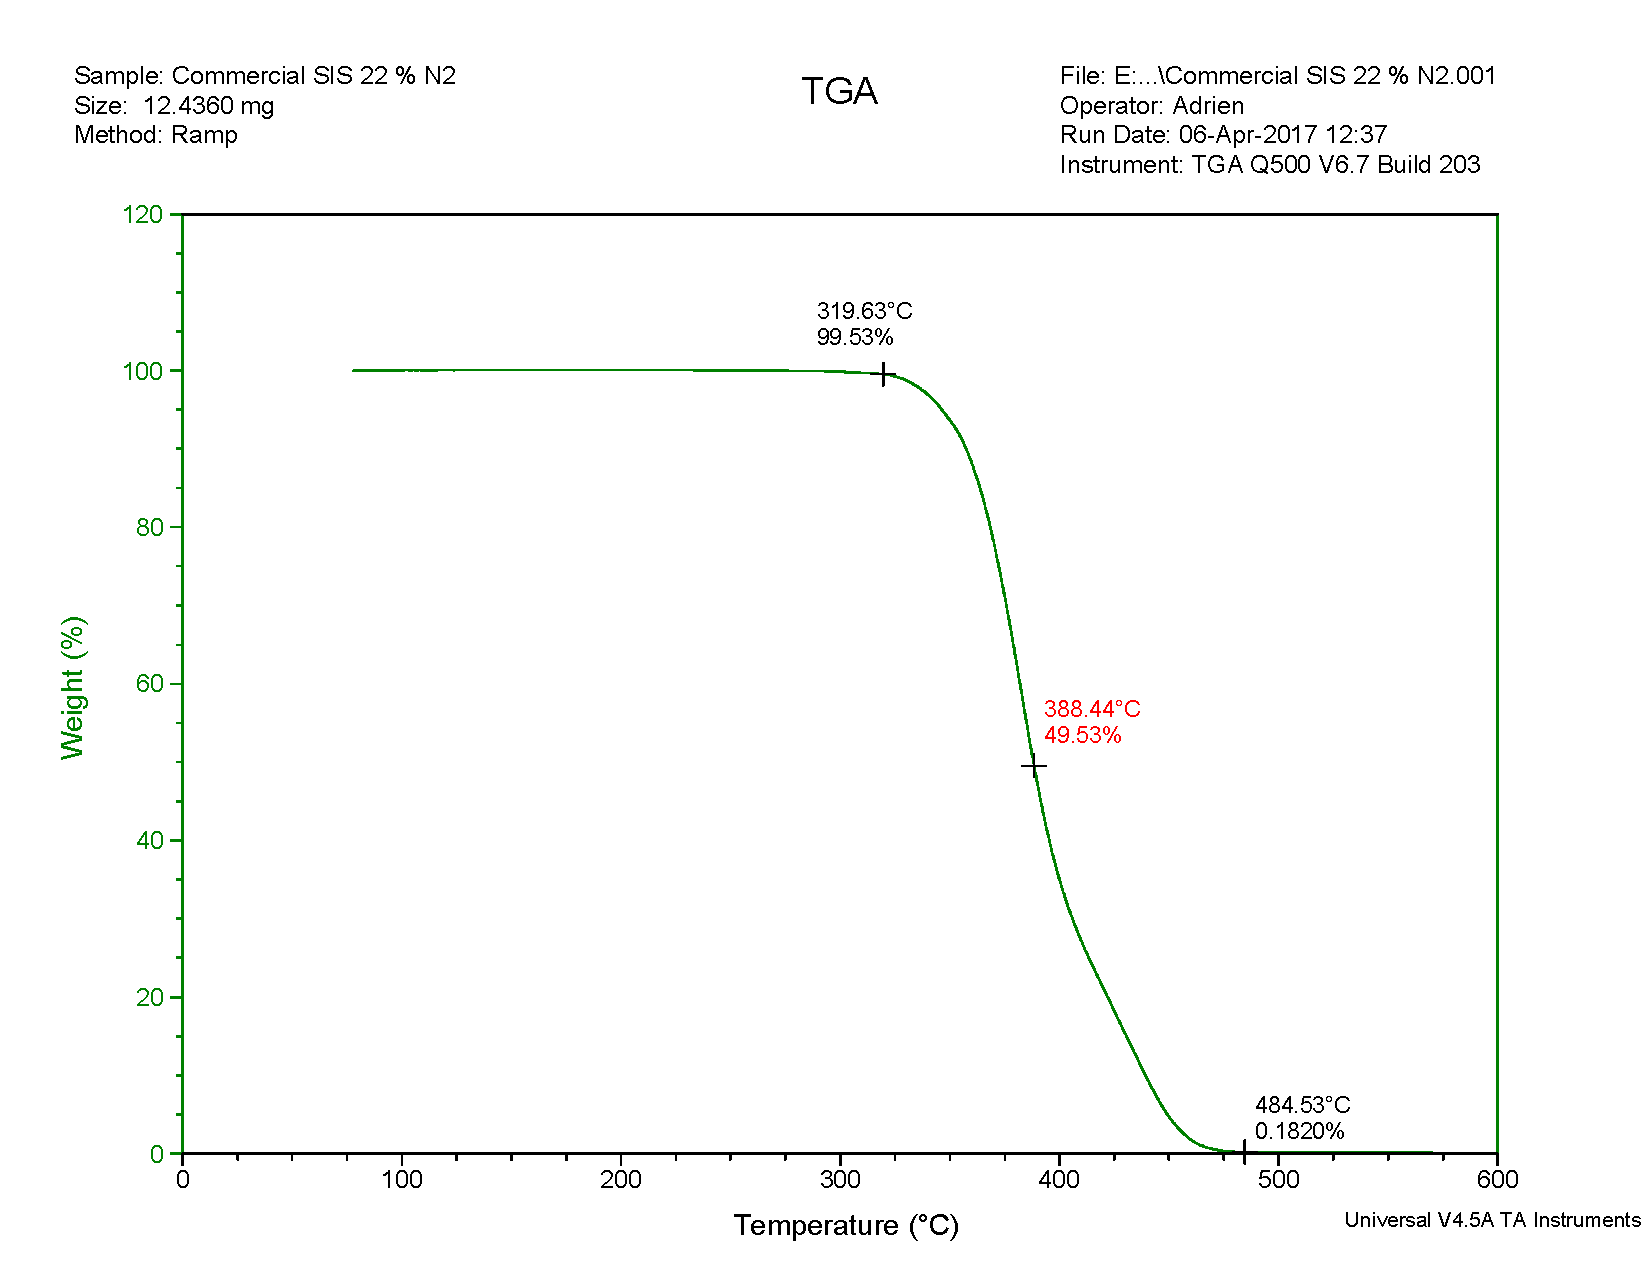
\includegraphics[width=0.75\textwidth]{TGA_Commercial_SIS_22p100_N2.pdf}
	}\\
	\subfigure[]
	{\label{fig:TGA_SYS_hydrogenated}
		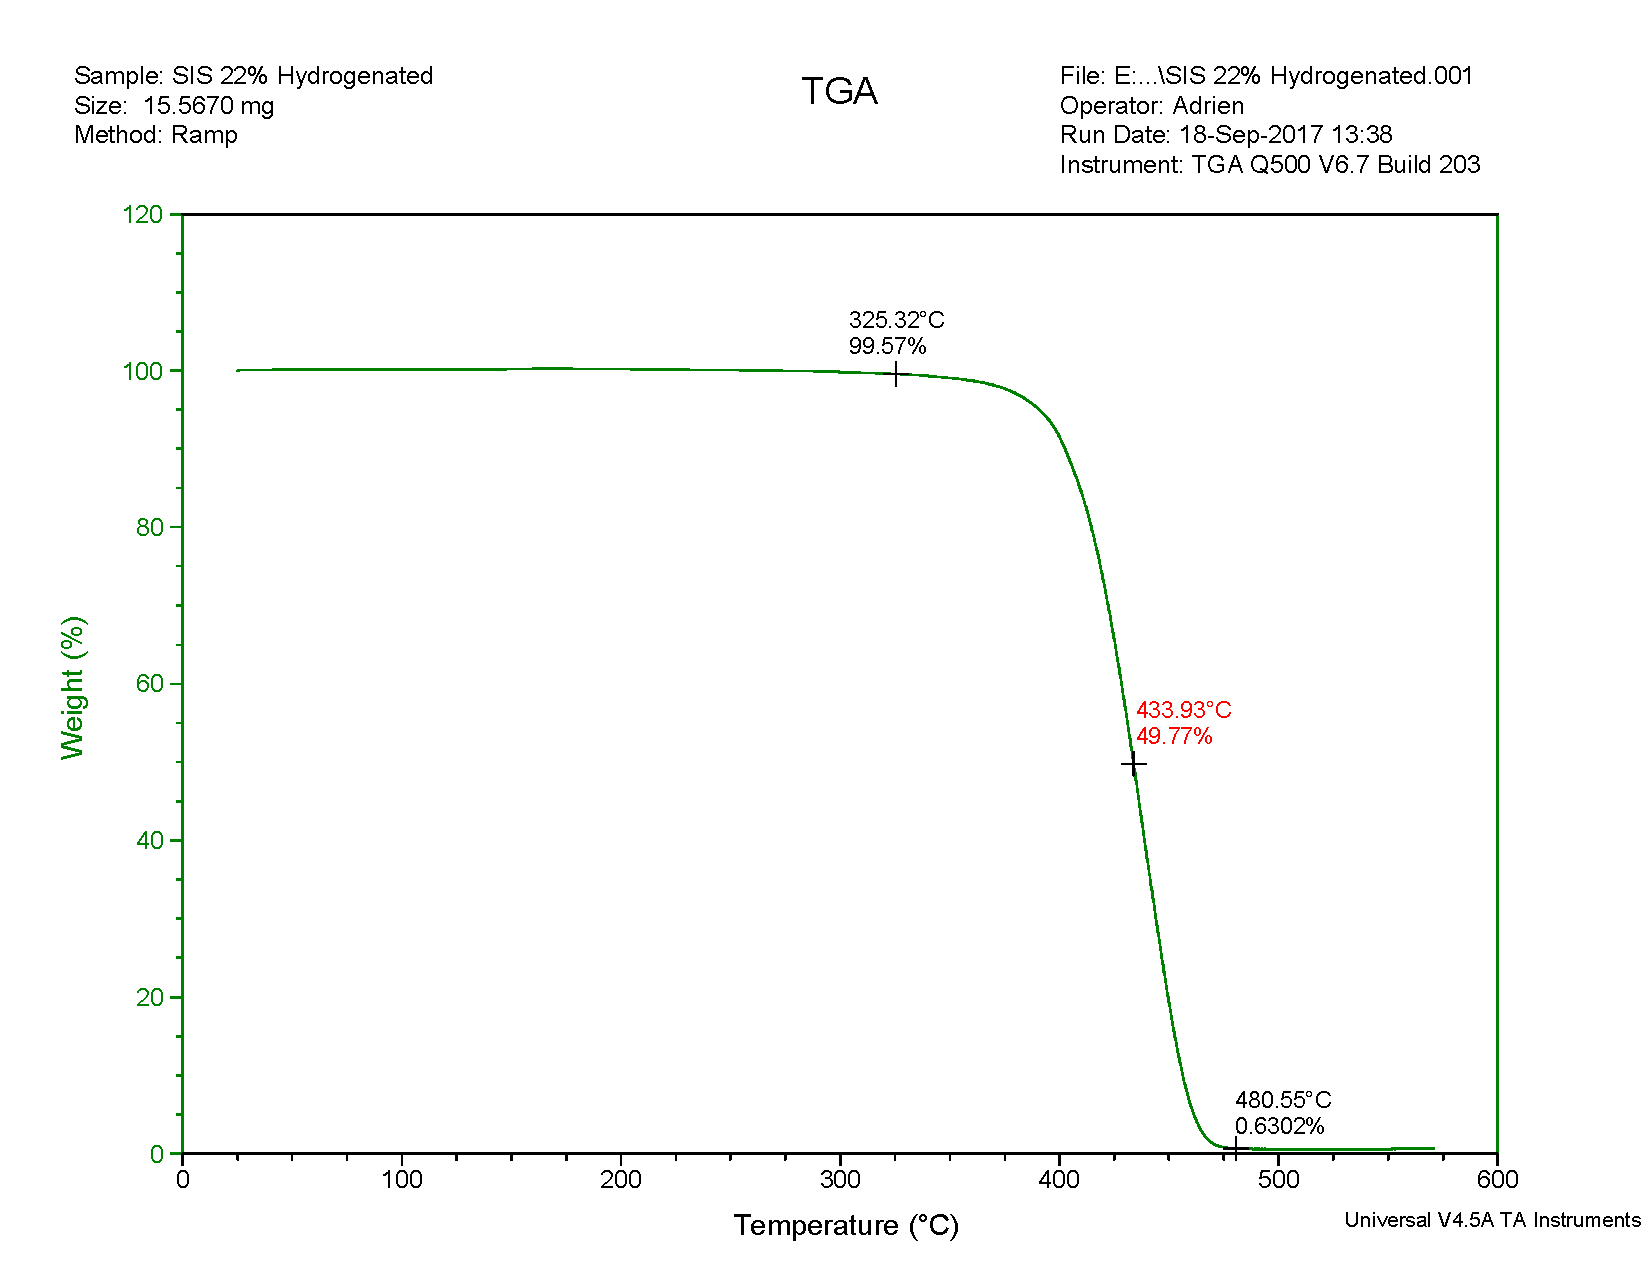
\includegraphics[width=0.75\textwidth]{TGA_Commercial_SIS_22p100_Hydrogenated_N2.pdf}
	}
	\caption{Résultats en TGA sous une atmosphère d'azote pour l'élastomère SIS commercial avec 22\% de styrène, a) SIS vierge, b) SIS ayant subi un traitement d'hydrogénation}
	\label{fig:TGA_SIS}
\end{figure}

En second lieu, le copolymère linéaire tribloc SEBS a été évalué. 
Les essais sous atmosphère standard (Fig. \ref{fig:TGA_rampe_SEBS_air}) ont démontré une dégradation rapide au-dessus de \SI[locale=FR]{270}{\celsius}. 
Cependant, puisque l'élastomère du joint n'est pas exposé directement à l'atmosphère durant le soudage, des essais sous atmosphère d'azote ont également été réalisés. 
Dans ces conditions, le SEBS a démontré une meilleure stabilité thermique que le SIS (Fig. \ref{fig:TGA_rampe_SEBS_N2}) avec des signes de dégradation observables seulement au-dessus de \SI[locale=FR]{340}{\celsius}. 

\begin{figure}[h]
	\centering
	\subfigure[]
	{\label{fig:TGA_rampe_SEBS_air} 								
		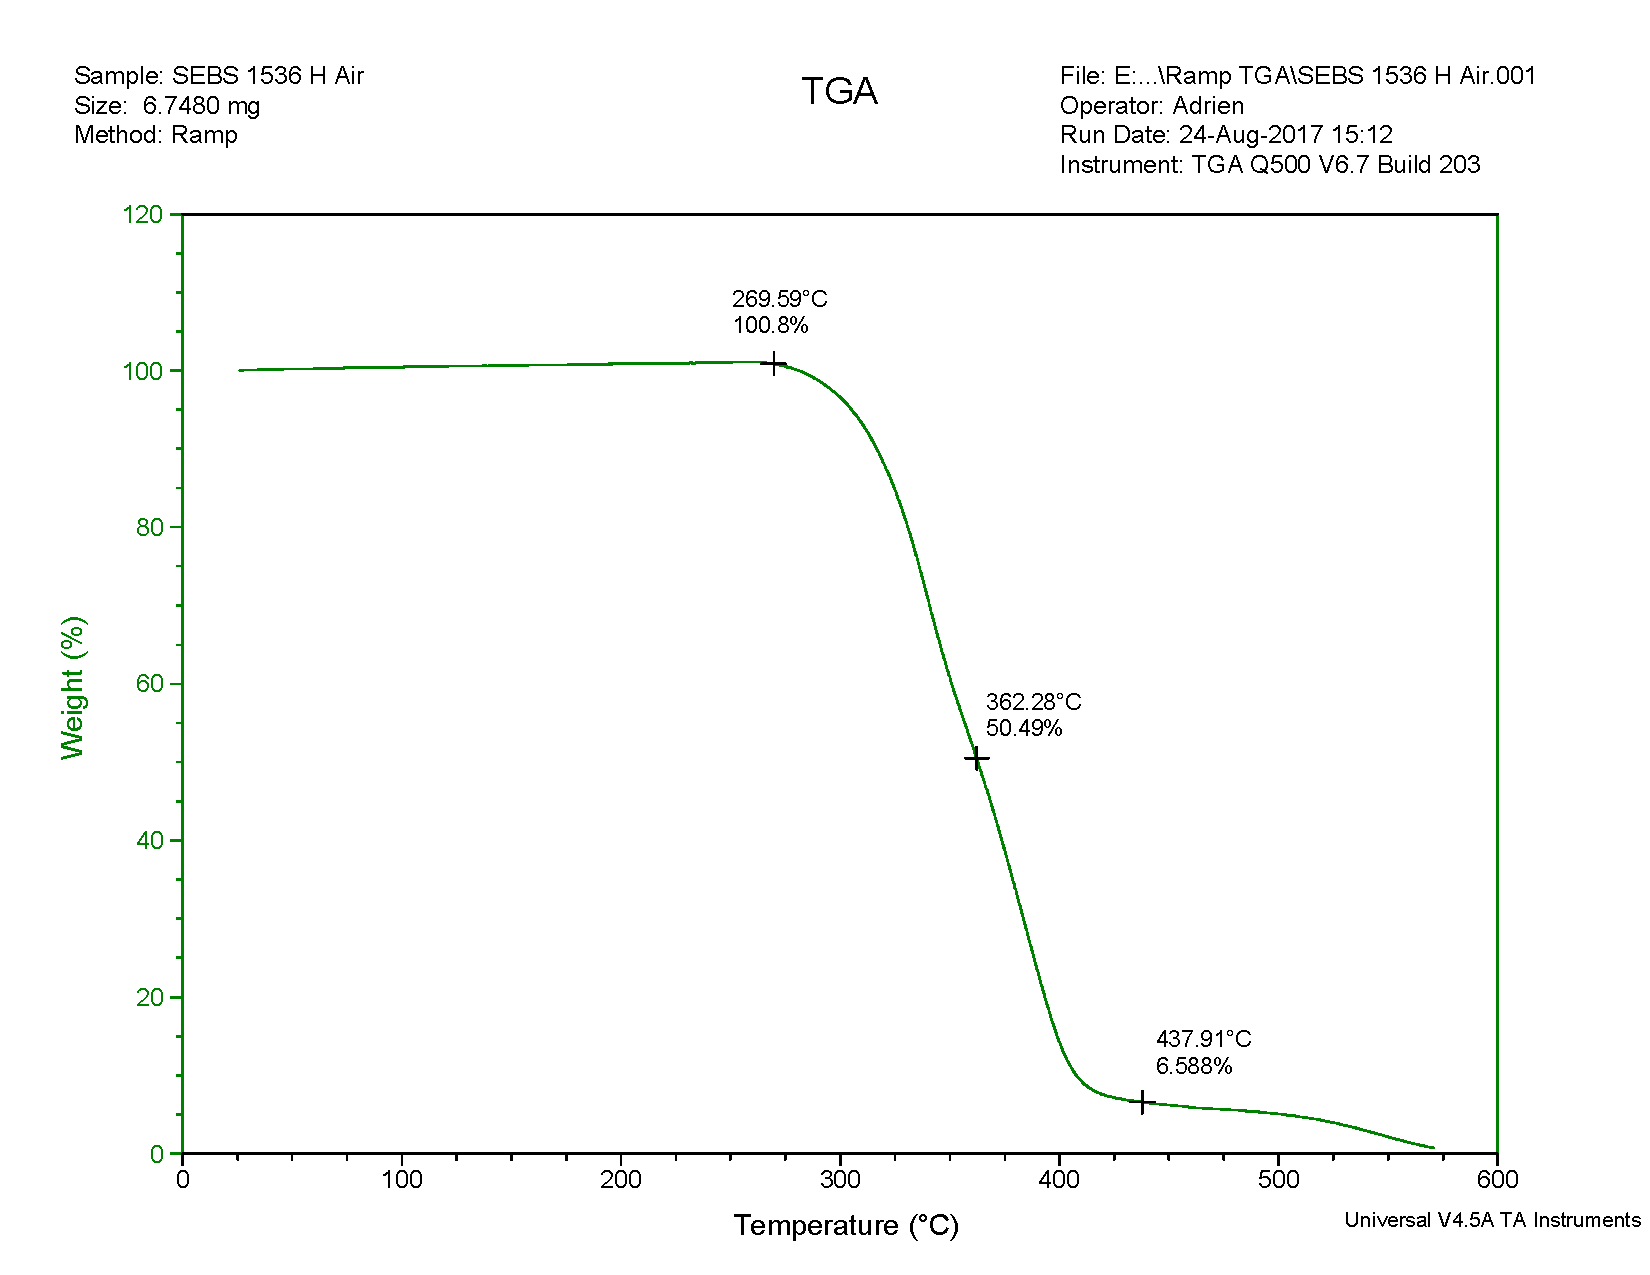
\includegraphics[width=0.75\textwidth]{TGA_SEBS_1536H_Air.pdf}
	}\\
	\subfigure[]
	{\label{fig:TGA_rampe_SEBS_N2}
		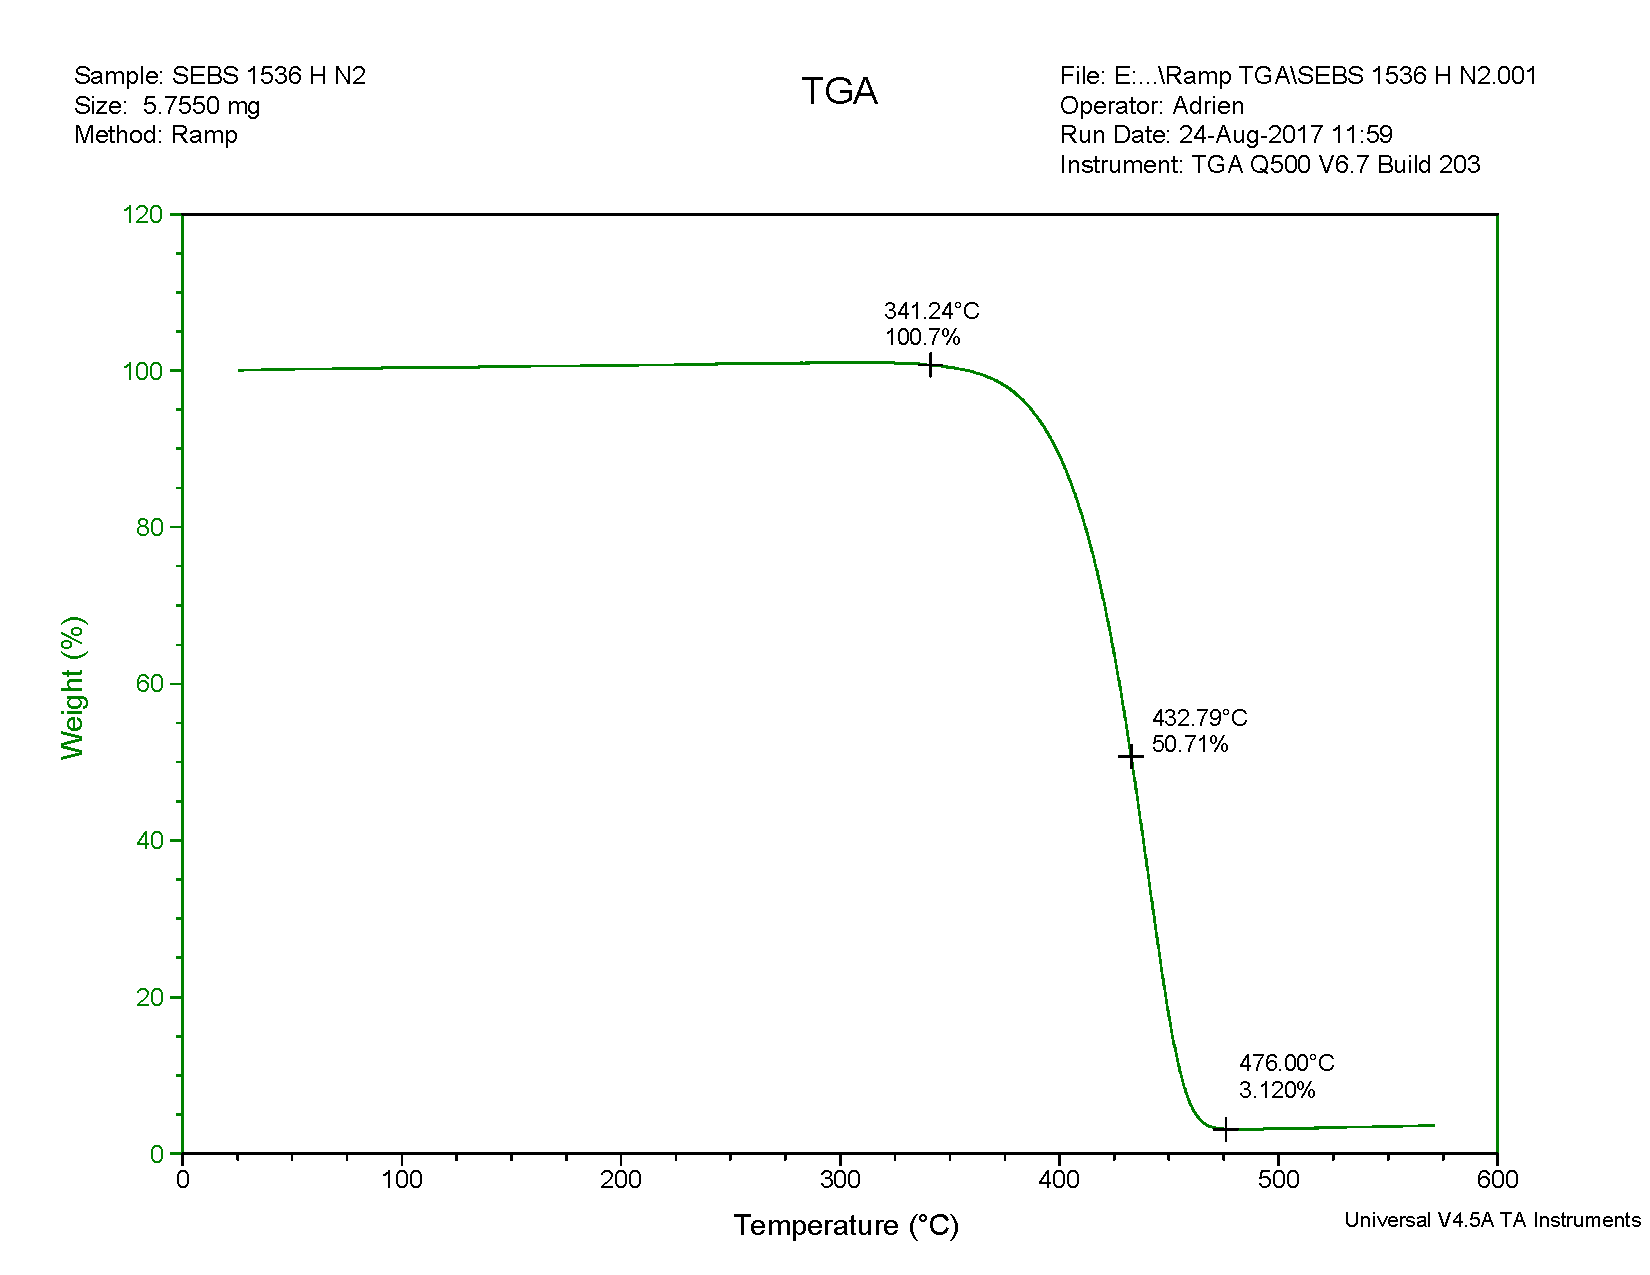
\includegraphics[width=0.75\textwidth]{TGA_SEBS_1536H_N2.pdf}
	}
	\caption{Résultats en TGA l'élastomère SEBS dans une atmosphère a) d'air, b) d'azote}
	\label{fig:TGA_rampe_SEBS}
\end{figure}

Il a été décidé de pousser plus loin l'analyse thermique de cet élastomère avec des essais de TGA isotherme. 
Les essais en isotherme sont beaucoup plus demandants que les essais standards avec une rampe de température. 
Cette méthode de test permet de valider hors de tout doute la stabilité thermique d'un polymère. 
Lorsque le test est réalisé avec une atmosphère standard (Fig. \ref{fig:TGA_iso_SEBS_air}), on observe une bonne stabilité thermique à \SI[locale=FR]{200}{\celsius} (Fig. \ref{fig:TGA_iso_SEBS_air_200}), mais on observe une dégradation thermique lente quand on répète l'essai à \SI[locale=FR]{230}{\celsius} (Fig. \ref{fig:TGA_iso_SEBS_air_230}). 
Quand cet essai est plutôt réalisé sous une atmosphère d'azote (Fig. \ref{fig:TGA_iso_SEBS_N2}), on observe des températures de dégradation légèrement plus élevées. 
Le SEBS est stable lorsqu'il est soumis à une température de \SI[locale=FR]{275}{\celsius} (Fig. \ref{fig:TGA_iso_SEBS_N2_275}), mais il commence à se dégrader lorsqu'il est soumis à une température de \SI[locale=FR]{290}{\celsius} (Fig. \ref{fig:TGA_iso_SEBS_N2_290}). 

\begin{figure}[h]
	\centering
	\subfigure[]
	{\label{fig:TGA_iso_SEBS_air_200} 								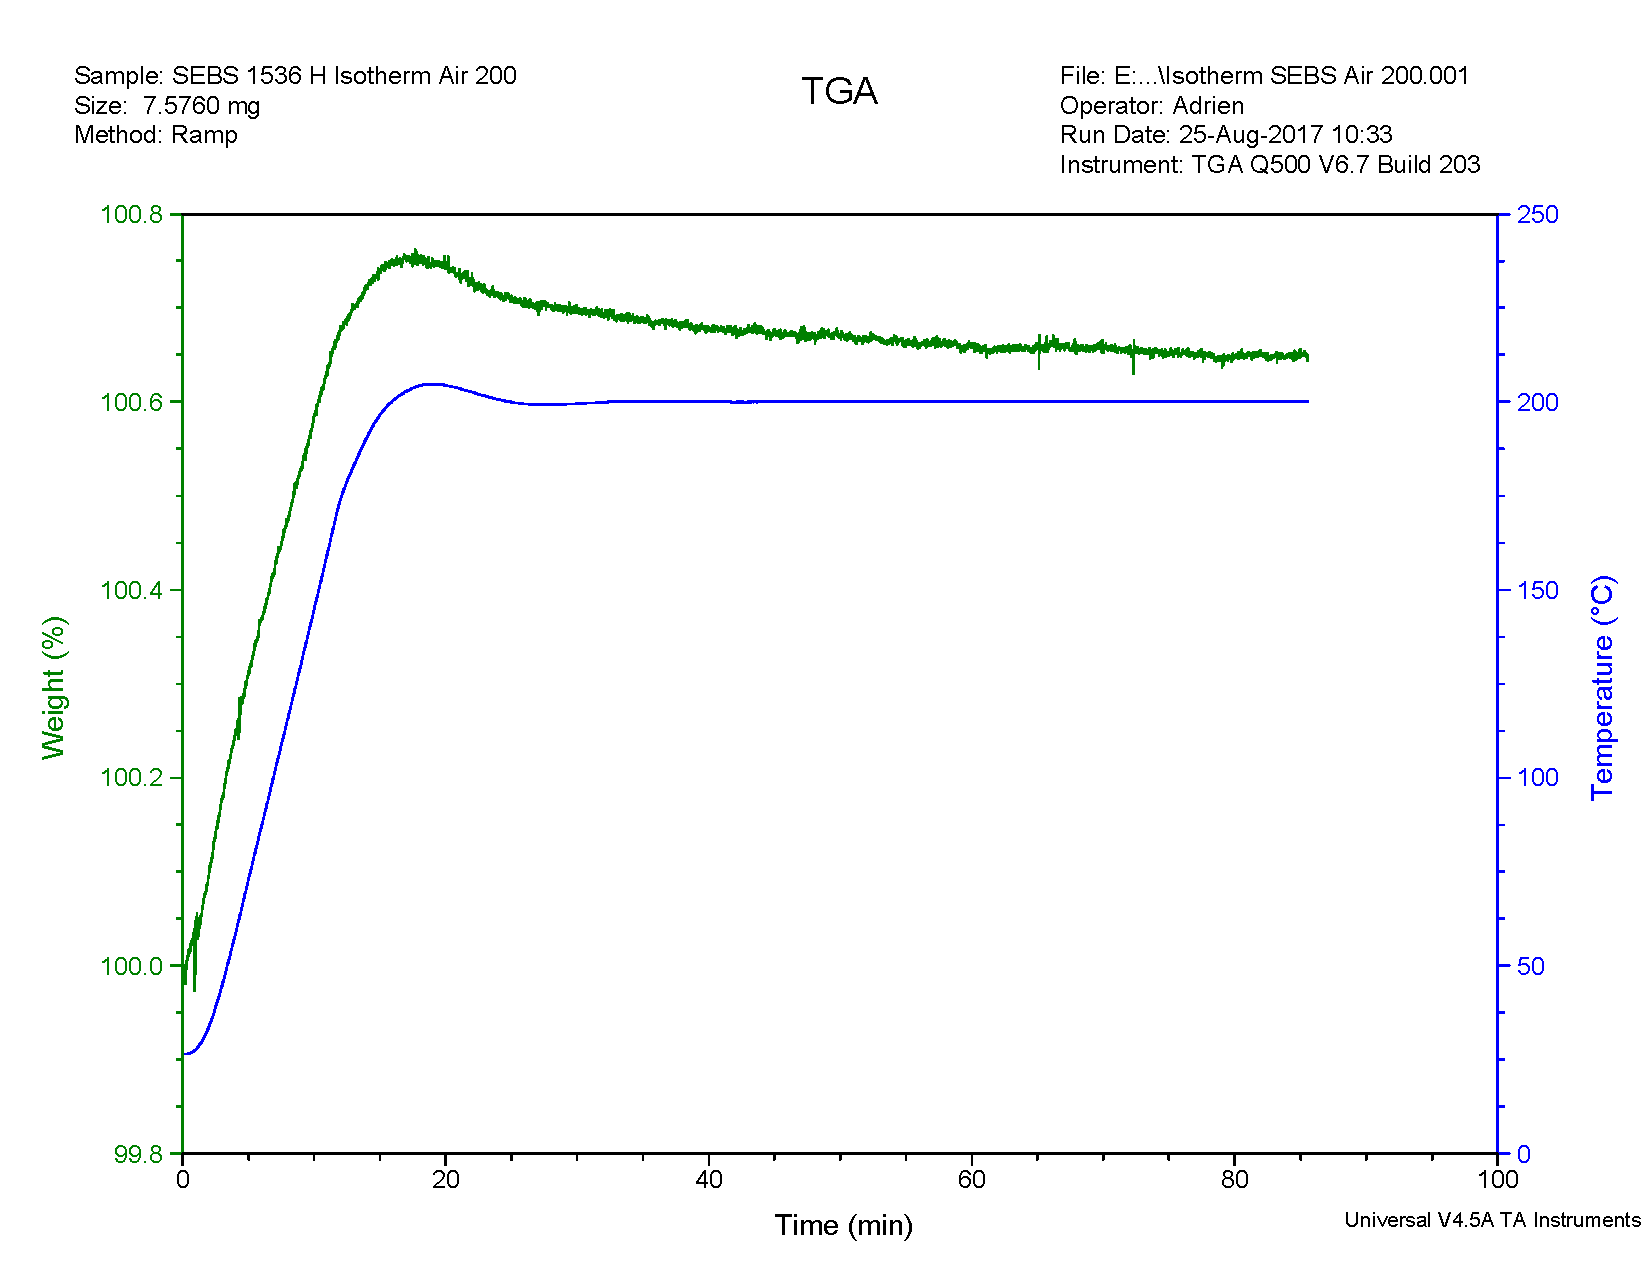
\includegraphics[width=0.75\textwidth]{TGA_SEBS_1536H_Air_Isotherm_200.pdf}
	}\\
	\subfigure[]
	{\label{fig:TGA_iso_SEBS_air_230}
		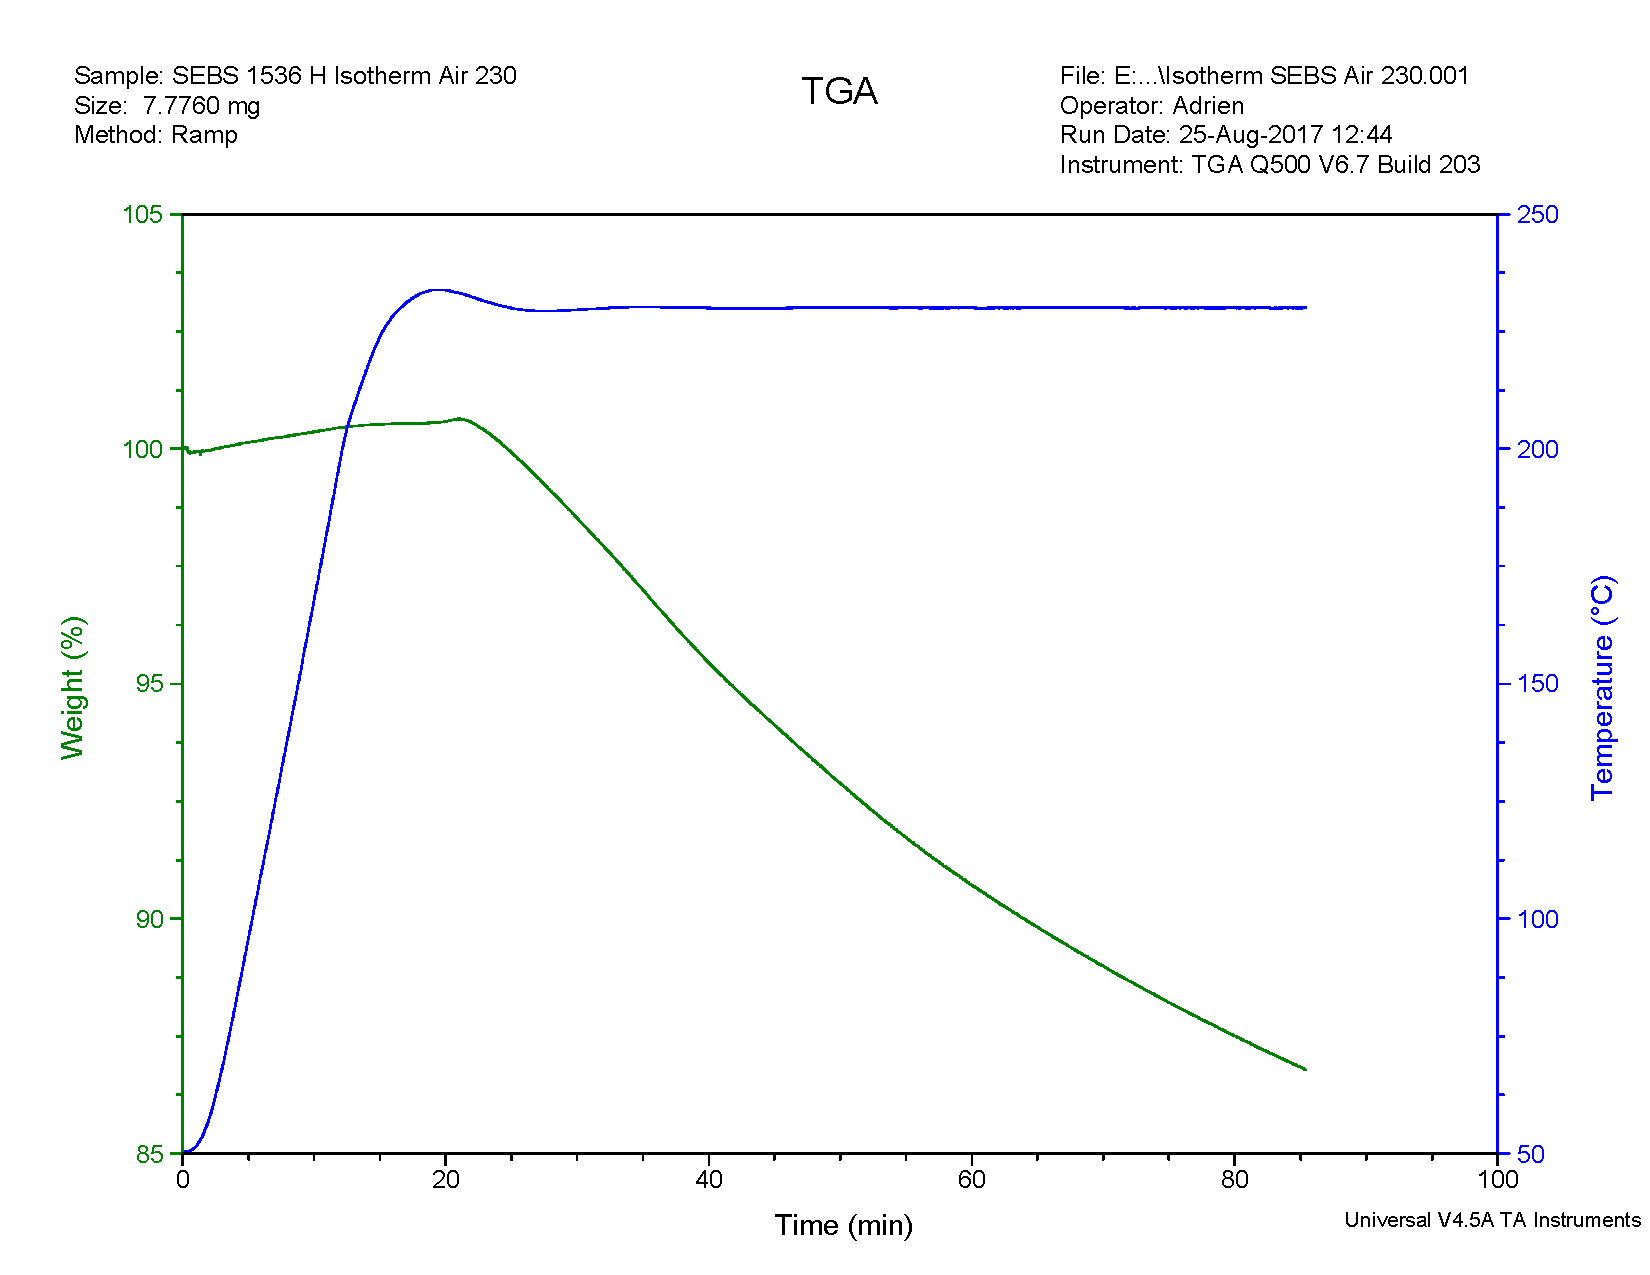
\includegraphics[width=0.75\textwidth]{TGA_SEBS_1536H_Air_Isotherm_230.pdf}
	}
	\caption{Résultats en TGA isotherme pour l'élastomère SEBS dans l'air à a) \SI{200}{\celsius} at b) \SI{230}{\celsius}}
	\label{fig:TGA_iso_SEBS_air}
\end{figure}

\begin{figure}[h]
	\centering
	\subfigure[]
	{\label{fig:TGA_iso_SEBS_N2_275} 								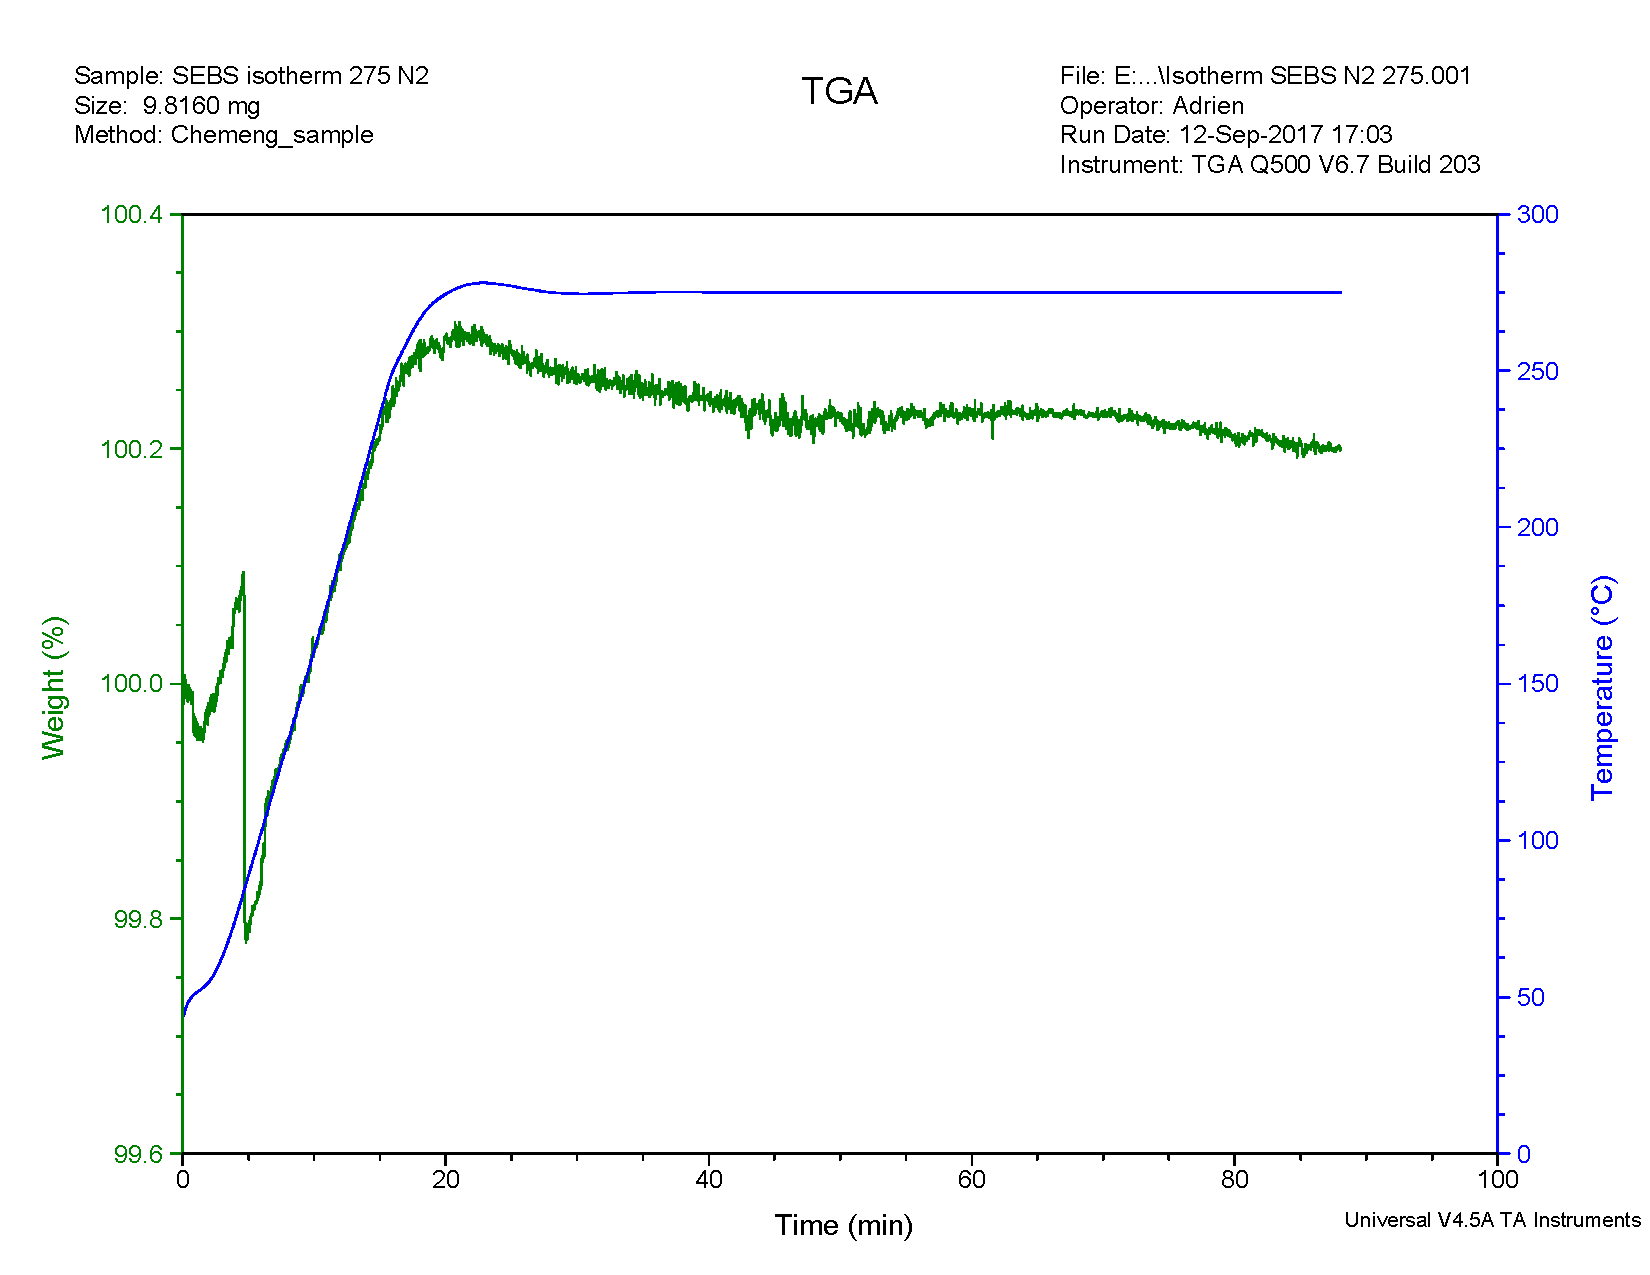
\includegraphics[width=0.75\textwidth]{TGA_SEBS_1536H_N2_Isotherm_275.pdf}
	}\\
	\subfigure[]
	{\label{fig:TGA_iso_SEBS_N2_290}
		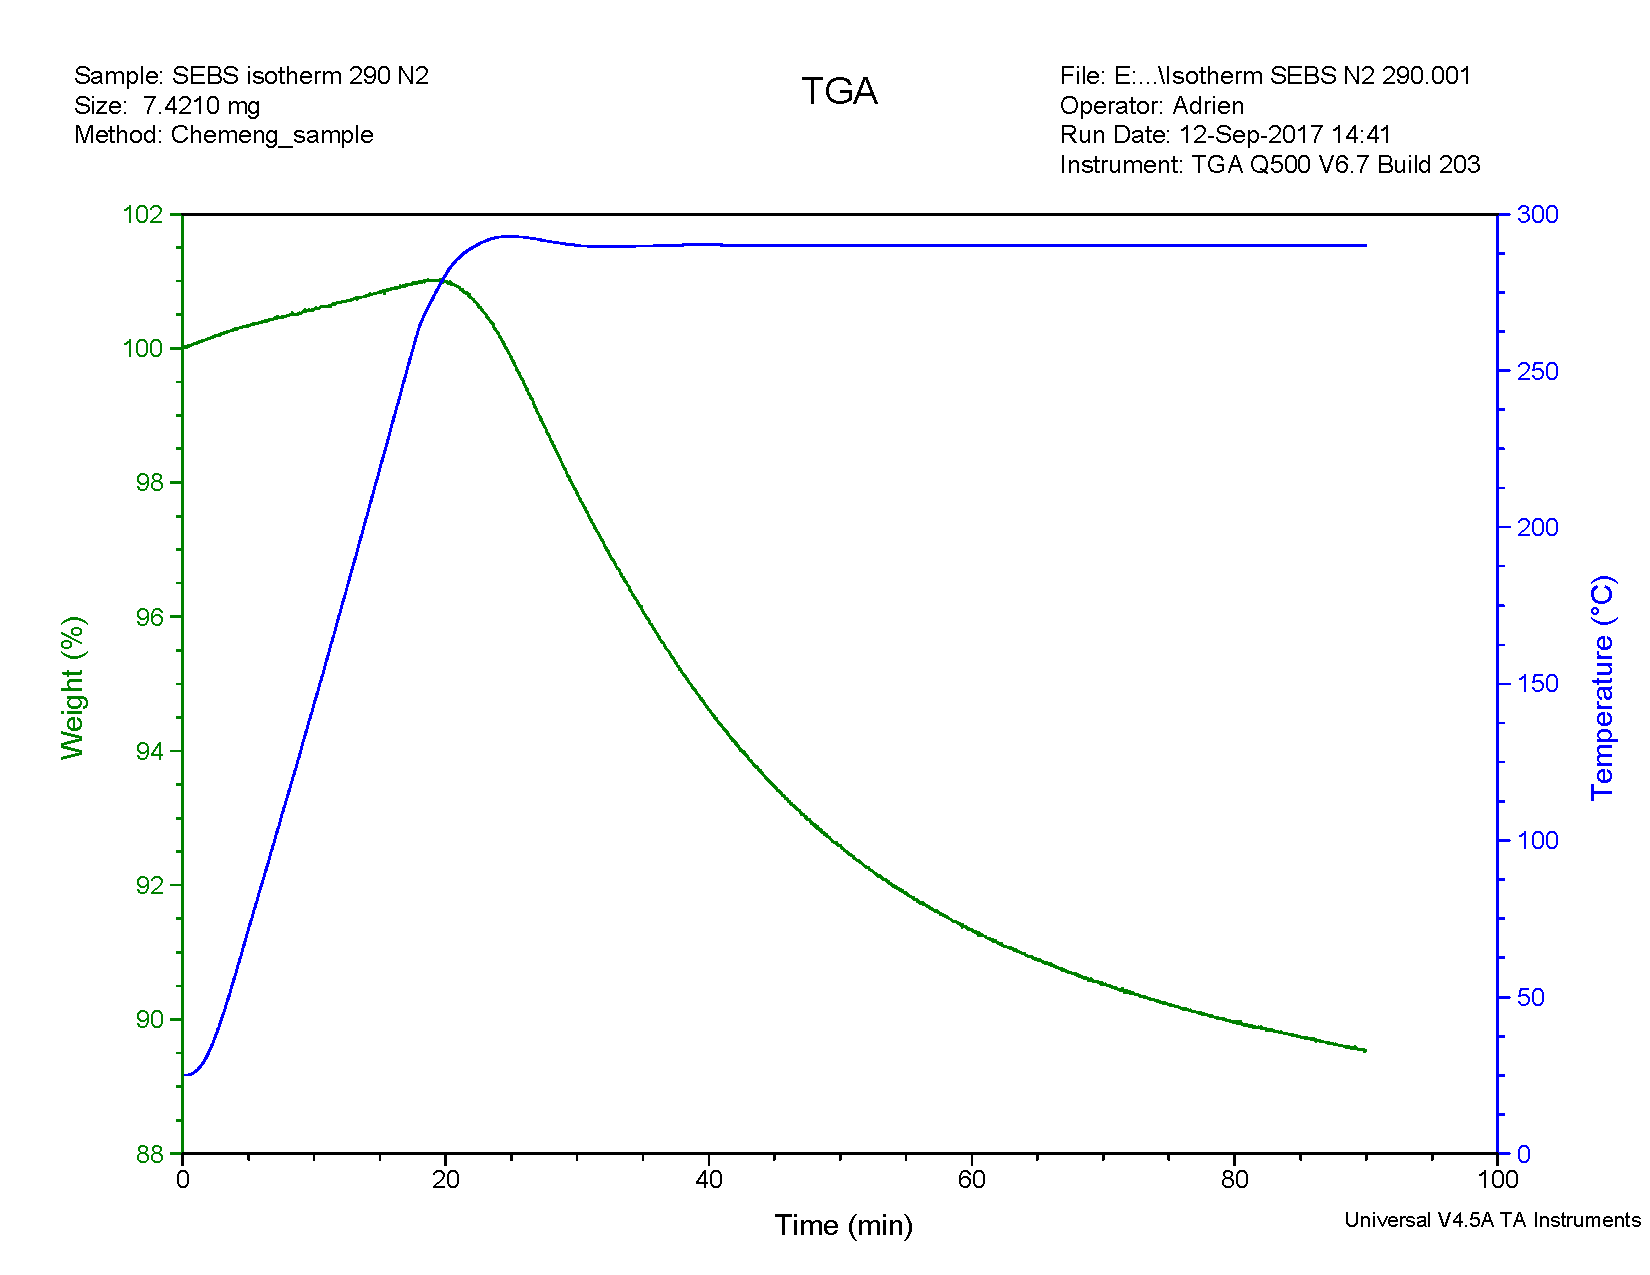
\includegraphics[width=0.75\textwidth]{TGA_SEBS_1536H_N2_Isotherm_290.pdf}
	}
	\caption{Résultats en TGA isotherme pour l'élastomère SEBS sous une atmosphère d'azote à a) \SI{275}{\celsius} at b) \SI{290}{\celsius}}
	\label{fig:TGA_iso_SEBS_N2}
\end{figure}

\section{Essais de soudage isotherme}

La stabilité thermique de l'élastomère SEBS a été jugée suffisamment bonne pour tenter de réaliser des jonctions soudées. 
Les premiers essais de soudage ont été réalisés dans une étuve sous vide en isotherme afin d'éviter de dégrader l'élastomère et de donner aux chaînes de polymère une longue période de temps afin qu'elles aient le temps de migrer au travers de l'interface. 
Lors du premier test, l'échantillon (Fig. \ref{fig:weldstack_SEBS}) dans l'étuve a été chauffé jusqu'à une température de \SI[locale=FR]{260}{\celsius}, pendant 24 heures. 
Les résultats obtenus démontrent le manque de tenue en température de l'élastomère et qu'un temps de soudage trop élevé lui permet de fluer en dehors de la zone à souder (Fig. \ref{fig:etuve_SEBS_flat}). 
De plus, dans la zone où de l'élastomère était encore en contact avec le nanocomposite, il était facile de le peler (Fig. \ref{fig:etuve_SEBS_pelage}). 
Ce test n'a pas été jugé totalement concluant puisqu'en raison du fluage de l'élastomère, la pression sur ce dernier n'était pas uniforme durant le test. 
La faible pression pourrait avoir nui au processus de diffusion des chaînes. 

\begin{figure}[h!]
	\centering
	\subfigure[]
	{\label{fig:weldstack_SEBS} 								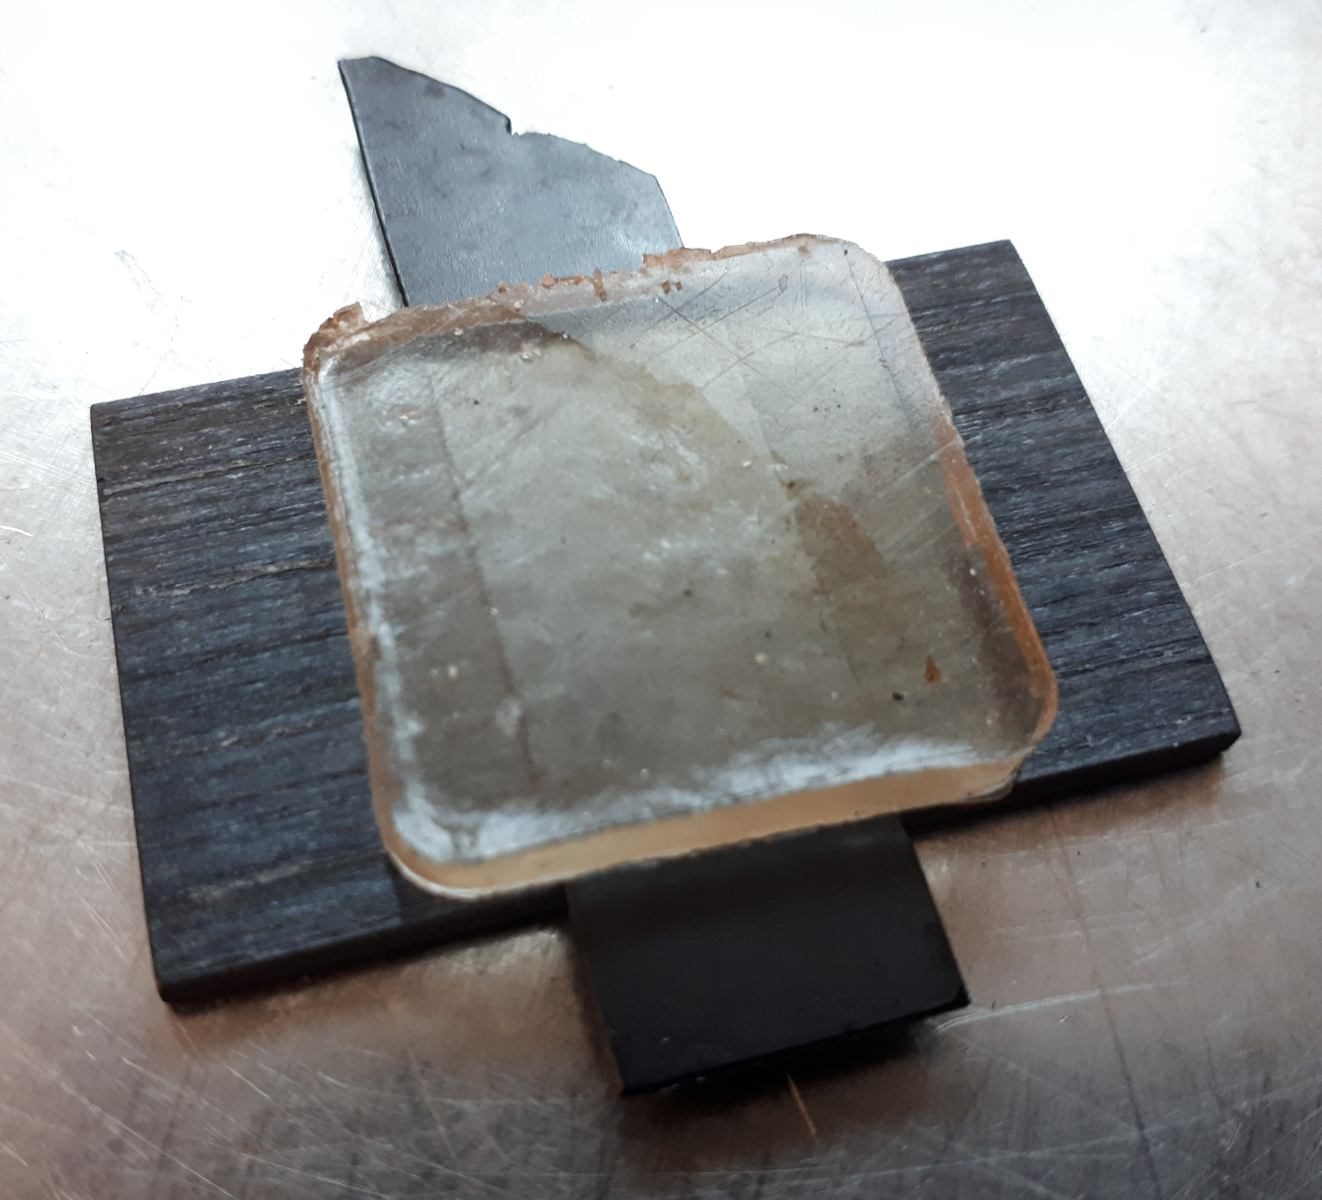
\includegraphics[height=4.2cm]{20171215_091800_crop_resize.jpg}
	} \
	\subfigure[]
	{\label{fig:etuve_SEBS_flat} 								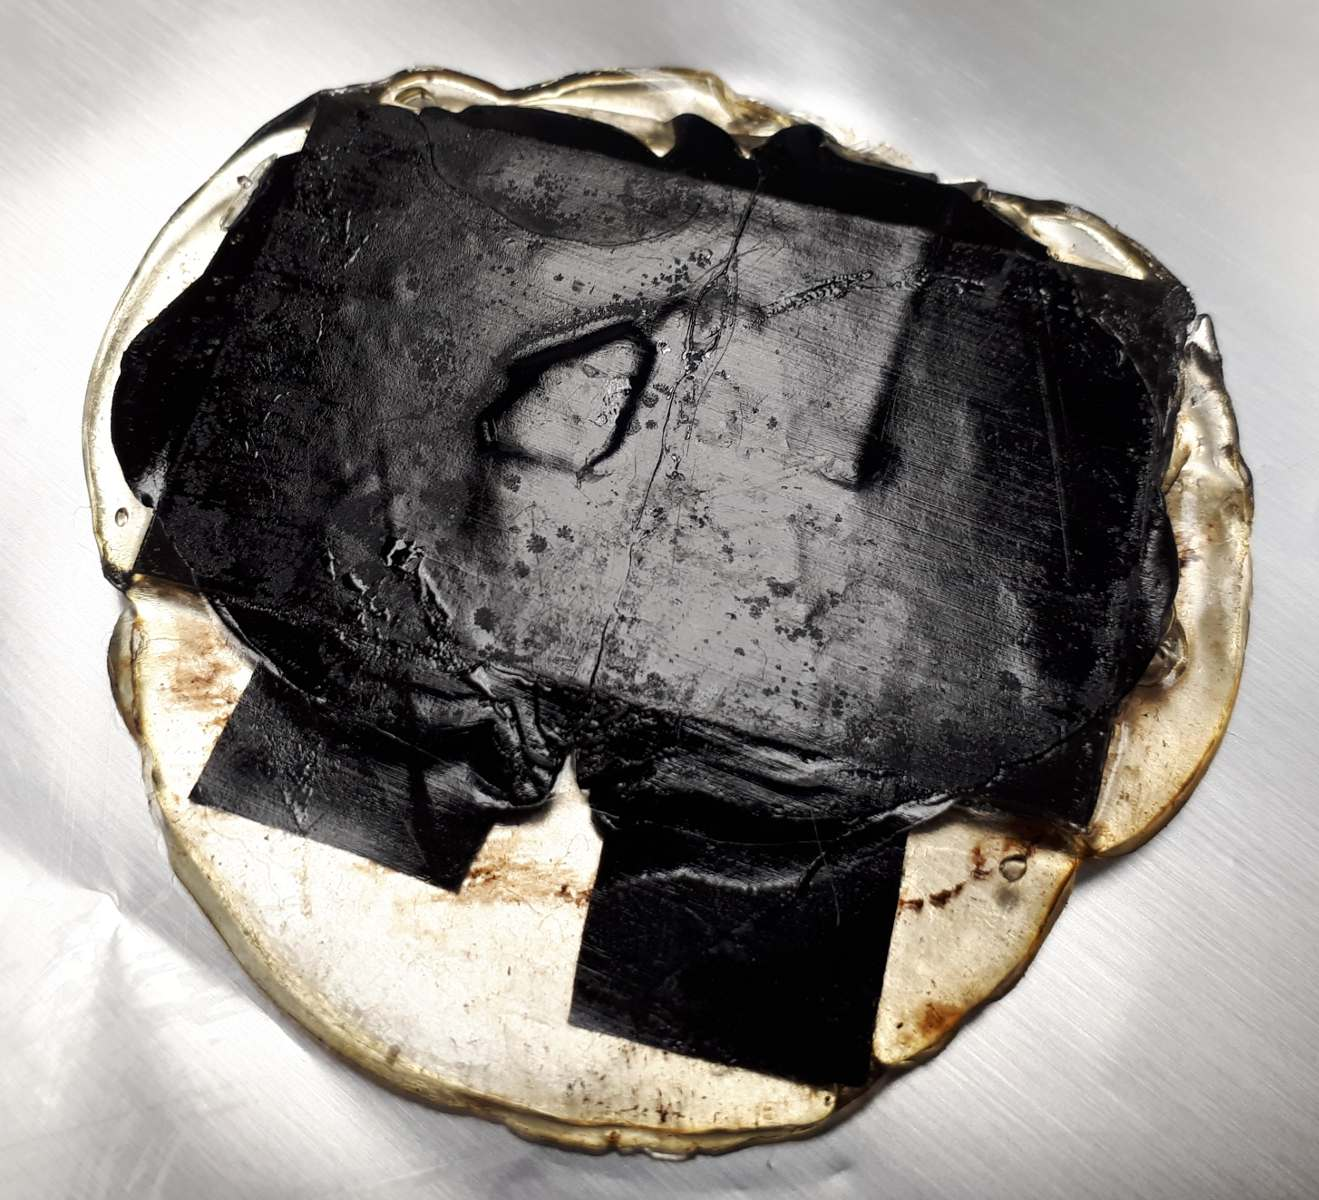
\includegraphics[height=4.2cm]{20180117_153151_crop_resize.jpg}
	} \
	\subfigure[]
	{\label{fig:etuve_SEBS_pelage}
		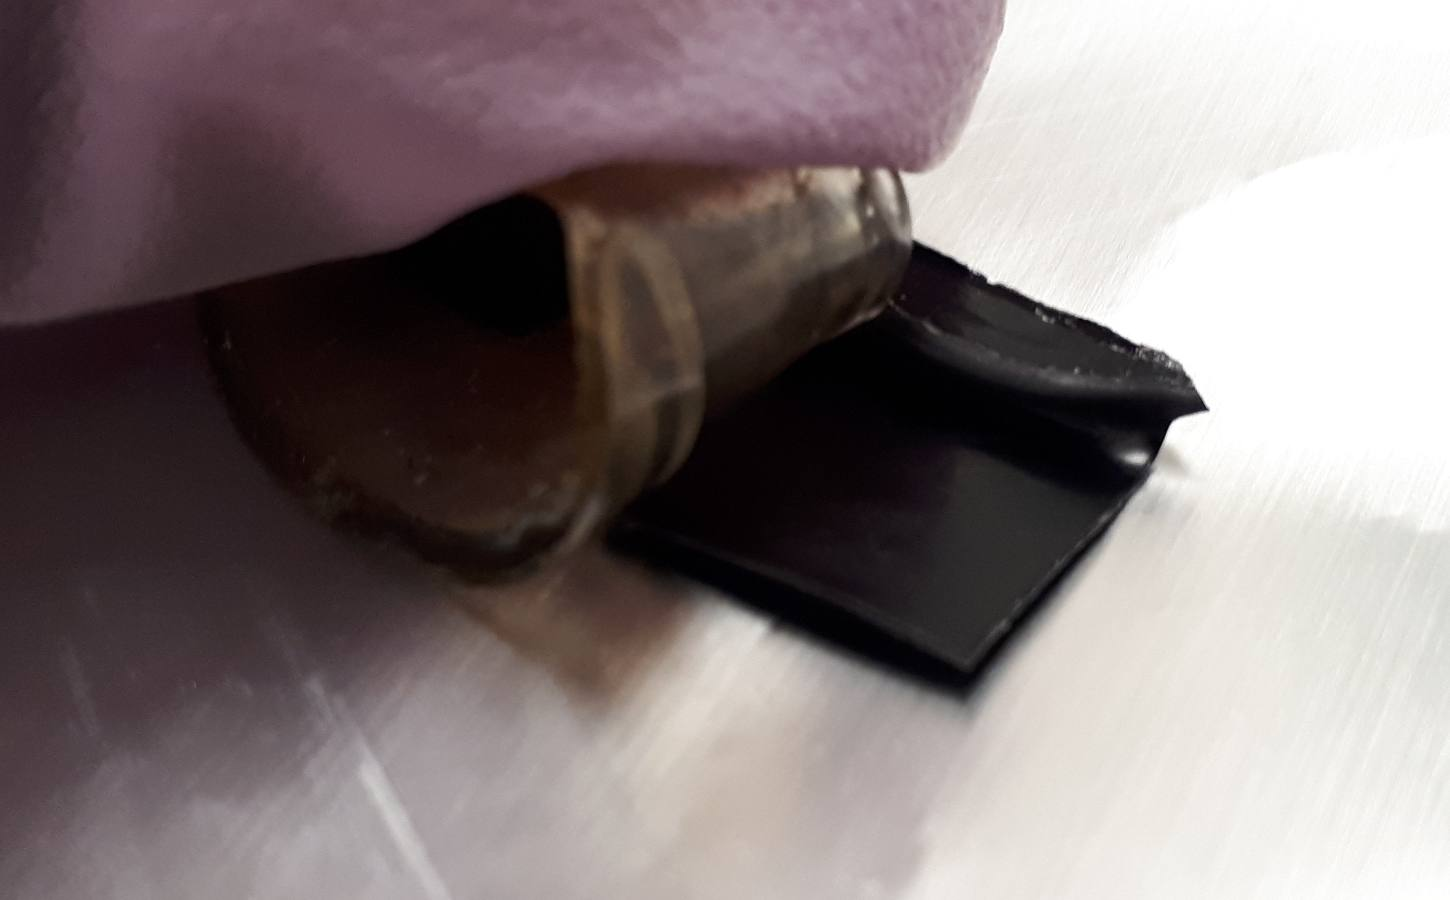
\includegraphics[height=3.5cm]{20180117_154300_crop_resize.jpg}
	}
	\caption{Essai de soudage dans une étuve sous vide à \SI{260}{\celsius} pour l'élastomère SEBS présentant a) la préparation de l'échantillon, b) l'échantillon à la sortie de l'étuve et c) le pelage de l'élastomère}
	\label{fig:etuve_SEBS}
\end{figure}

\begin{figure}[h]
	\centering
	\subfigure[]
	{\label{fig:welds_SEBS_presse} 								
		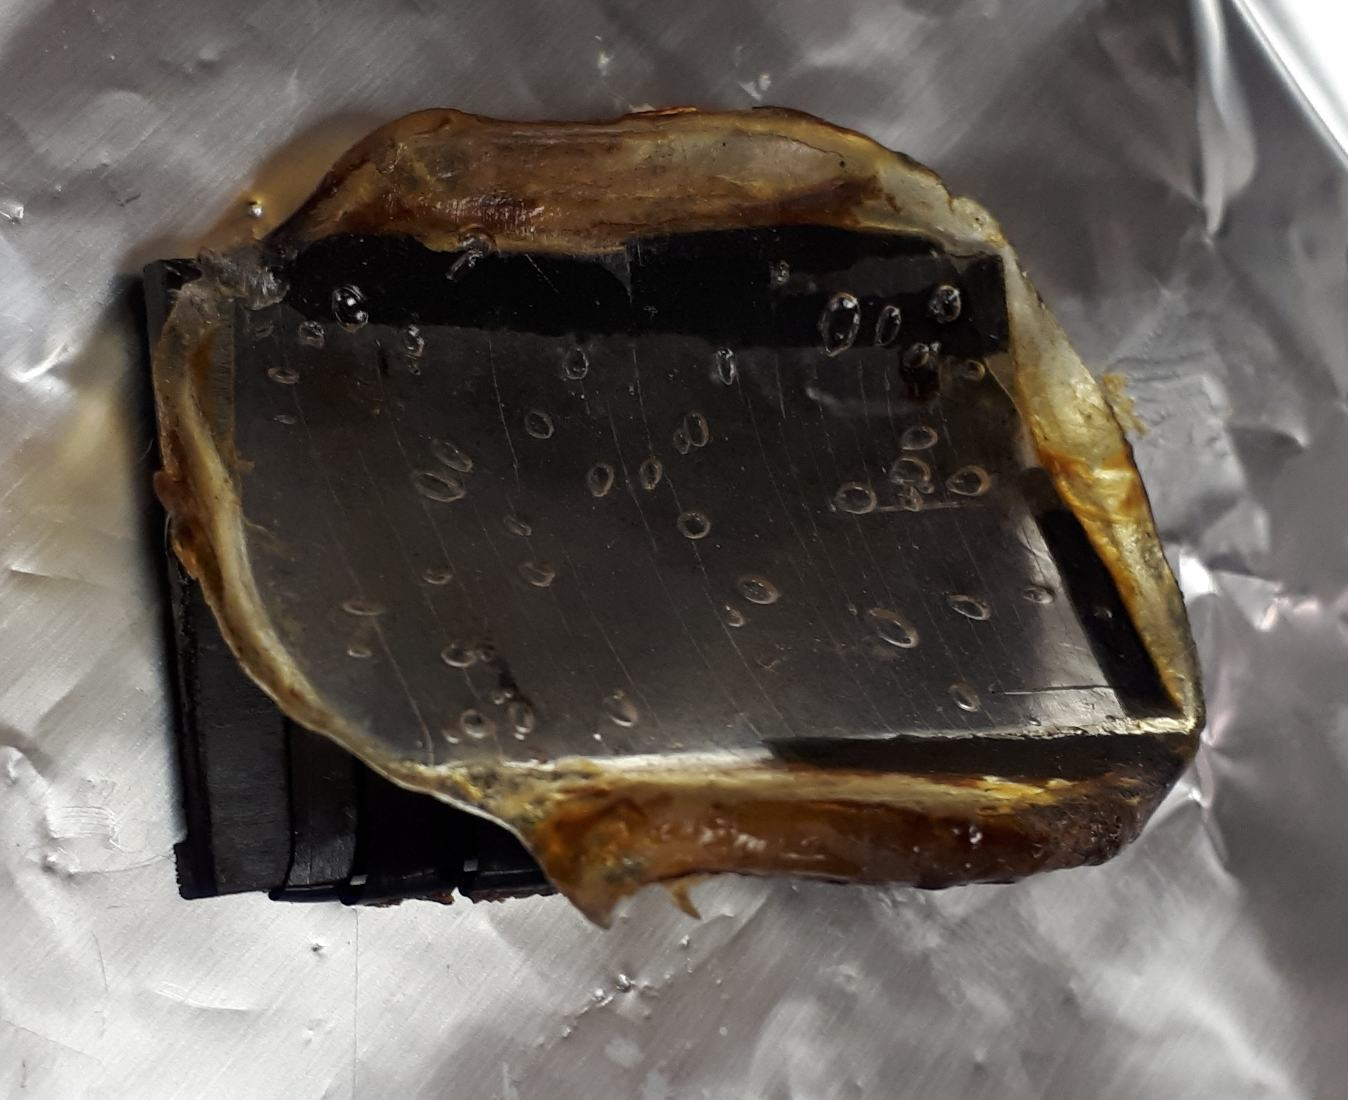
\includegraphics[height=6.cm]{20180124_142710_crop_resize.jpg}
	} \qquad
	\subfigure[]
	{\label{fig:welds_SEBS_presse_pelage} 								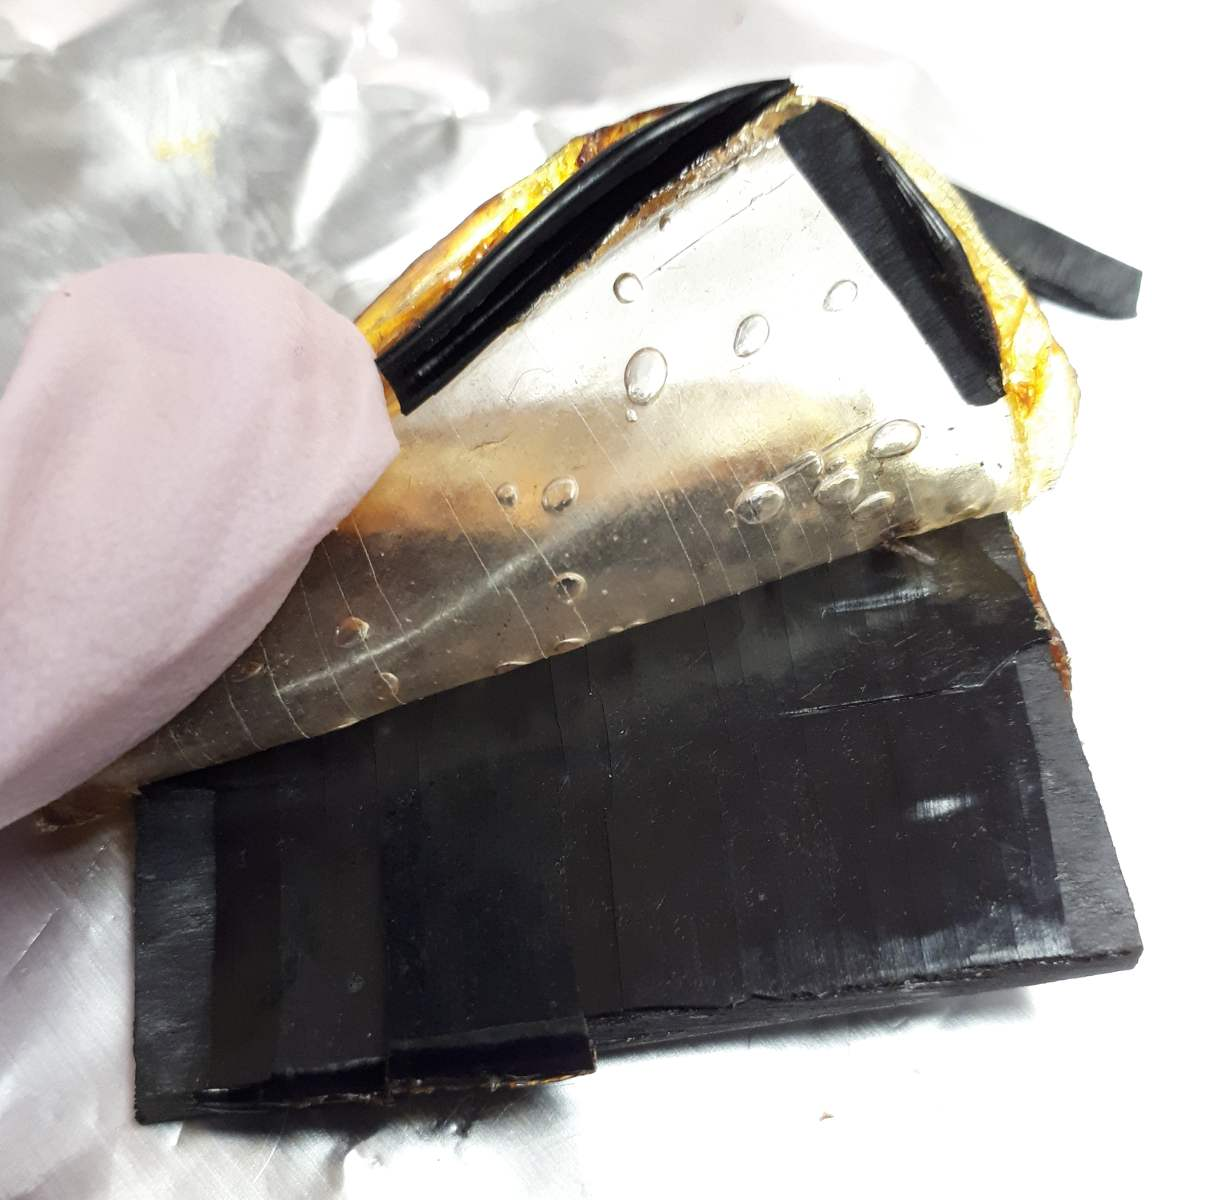
\includegraphics[height=6.cm]{20180124_142724_crop_resize.jpg}
	}
	\caption{Essai de soudage à la presse à \SI{260}{\celsius} pour l'élastomère SEBS présentant a) l'échantillon à la sortir de la presse et b) le pelage de l'élastomère}
	\label{fig:presse_SEBS}
\end{figure}

\FloatBarrier
Suite aux premiers résultats à l'étuve, il a été décidé de réaliser un essai de soudage à la presse chauffante avec l'élastomère SEBS. 
Cet essai avait pour but de tenter un temps de soudage plus court, mais avec une pression de contact plus élevée. 
Cependant, la force minimale que la presse a pu appliquer durant ce test a causé une pression de \SI[locale=FR]{5}{\mega\pascal} qui a entrainé le fluage de l'élastomère (Fig. \ref{fig:welds_SEBS_presse}). 
Encore une fois, l'élastomère a pu être facilement séparé du nanocomposite (Fig. \ref{fig:welds_SEBS_presse_pelage}). 
En raison de l'ensemble des résultats obtenus pour le SEBS, les essais pour cette famille de polymère se sont conclus à ce point. 

%%%%%%%%%%%%%%%%%%%%%%%%%%%%%%%%%%%%%%%%%%%%%%%%%%%%%%%%%%%%%%%%%%
\Annexe{Informations complémentaires au chapitre 4}
%%%%%%%%%%%%%%%%%%%%%%%%%%%%%%%%%%%%%%%%%%%%%%%%%%%%%%%%%%%%%%%%%%

Le texte de cette annexe a été publié en accompagnement du premier article. 
Les modèles par éléments finis ont été développés afin de valider les mécanismes de génération de chaleur dans le nanocomposite. 

%%%%%%%%%%%%%%%%%%%%%%%%%%%%%%%%%%%%%%%%%%%%%%%%%%%%%%%%%%%%%%%%%
\section{Supplementary Information}
%%%%%%%%%%%%%%%%%%%%%%%%%%%%%%%%%%%%%%%%%%%%%%%%%%%%%%%%%%%%%%%%%

%%%%%%%%%%%%%%%%%%%%%%%%%%%%%%%%%%%%%%%%%%%%%%%%%%%%%%%%%%%%%%
\subsection{Continuum Micromechanic Simulations}
%%%%%%%%%%%%%%%%%%%%%%%%%%%%%%%%%%%%%%%%%%%%%%%%%%%%%%%%%%%%%%

In the early phase of the nanocomposite heating elements development, finite element models were developed using COMSOL Mul\-ti\-phy\-sics\-\textregistered \ to verify that the polymer would not undergo thermal degradation and to evaluate the contribution of the three main heating mechanisms inside the nanocomposite heating element (i.e. Joule heating of MWCNTs, from the concentration of charges at the contact points between MWCNTs and of the matrix between MWCNTs).  
A set of three continuum micromechanic models presenting different contact topologies were used to assess the relative contribution of each heating mechanism to the global heating phenomena within a conductive nanocomposite. 
Representative elementary volumes (REV) in which the MWCNTs represented 1\% of the total mass were used in these models (Fig. \ref{fig:geometry}). 

\begin{figure}[htb]
	\centering
	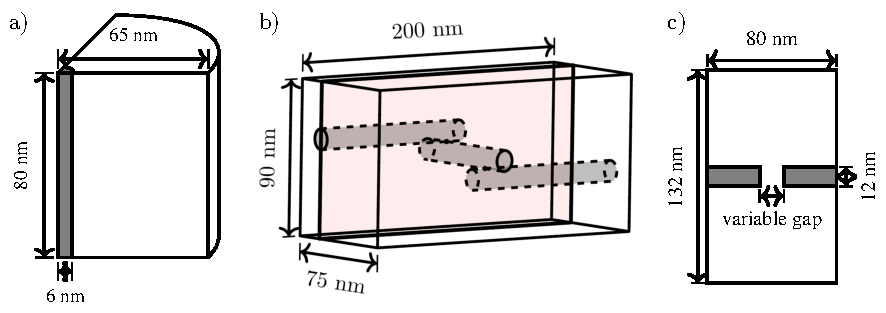
\includegraphics[width=150mm]{Fig1s.pdf}
	\caption{Geometries of the representative elementary volume composed of MWCNT (dark region) and the insulating matrix (white region) a) Quarter view of the revolved 2D axisymmetric FEM simulating the Joule heating within a MWCNT, b) Geometry of the second FEM evaluating the effect of charge concentration at contact point, c) Geometry of the third FEM simulating Joule heating within the polymer matrix \cite{Brassard2018_figshare_article1}}
	\label{fig:geometry}
\end{figure}

\FloatBarrier

In the first model, a single MWCNT (Fig. \ref{fig:geometry}a dark zone), surrounded by PEI (Fig. \ref{fig:geometry}a white zone) was represented using axisymmetric boundary conditions. 
The top and bottom surfaces of the MWCNT acted as voltage source and ground, respectively, with the current flowing through the MWCNT. 
The diameter of the MWCNT was set to \SI{12}{\nano\metre} in agreement with the data obtained from our supplier. 
This model assumed heat generation through Joule effect inside the MWCNT and heat transfer by conduction occurring radially from the MWCNT to the polymer.

In the second model, the flow of the current has to cross through direct contact between adjacent nanotubes. 
The REV (Fig. \ref{fig:geometry}b) includes three MWCNTs (dark region) that form a percolated electrical path within the polymer matrix. 
The current from the voltage source must transfer through two contact point interfaces to reach the ground on the other side of the conductive network. 
The highlighted plane shows the area of interest for temperature monitoring. 
Joule heating from within the MWCNTs was also present in this model. 

In the third model, the current was forced to flow through a polymer gap, of variable length, between two adjacent MWCNTs (Fig. \ref{fig:geometry}c). 

In each simulation, a constant DC electric field was applied for \SI{5}{\second} and the resulting temperature field was recorded. 
The value of the electric field was adjusted so as to reach similar temperatures after \SI{5}{\second} in all three models. 
A volumetric electromagnetic heat source was used to simulate Joule heating. 
Conductive heat transfer within solids (Fourier's law) is considered and the current is conserved within the REV (conservation law). 
Electrical insulation and symmetric thermal boundary conditions were set for the edges of the polymer matrix that were not in contact with the MWCNT. 
Symmetric thermal boundary conditions were defined at both ends of the MWCNT. 
These boundary conditions were selected to simulate a REV far from the outer surfaces of the nanocomposite heating element. 
Under these conditions, heat was generated within the three models but had no way to exit, causing the temperature to increase as energy kept accumulating.

The physical properties of PEI were used for the polymer matrix alongside physical properties for MWCNT taken from the literature (Tab. \ref{tab:material_properties}). 

\begin{table}[h]
	\center
	\caption{Material properties, unless noted, the properties for PEI are taken from SABIC's technical documentation}
	\resizebox{\textwidth}{!}{
		\begin{tabular}{@{}lllrlrl@{}}
			\toprule
			Property                &                   &                                         &         PEI &                     &       MWCNT &                           \\ \midrule
			Density                 & $\rho$            & [\si{\kilo\gram\per\cubic\metre}]       &        1270 &                     &        2000 & \cite{Lehman2011}         \\
			Specific heat           & $C_p$             & [\si{\joule\per\kilo\gram\per\celsius}] &        1248 & \cite{Ageorges2001} &         600 & \cite{Mizel99}            \\
			Thermal conductivity    & $k$               & [\si{\watt\per\metre\per\celsius}]      &        0.22 &                     &        3000 & \cite{Mizel99,Berber2000} \\
			Electrical conductivity & $\sigma$          & [\si{\siemens\per\metre}]               & \num{1e-15} &                     & \num{8.3e5} & \cite{Ebbesen1996}        \\
			Relative permittivity   & $\upvarepsilon_r$ & [ \hspace{0.5em} ]                      &        3.15 &                     &        12.5 & \cite{Katsounaros2011}    \\ \bottomrule
	\end{tabular}}
	\label{tab:material_properties}
\end{table}

%%%%%%%%%%%%%%%%%%%%%%%%%%%%%%%%%%%%%%%%%%%%%%%%%%%%%%%%%%%%%%
\FloatBarrier
\subsection{Simulations Results}
%%%%%%%%%%%%%%%%%%%%%%%%%%%%%%%%%%%%%%%%%%%%%%%%%%%%%%%%%%%%%%

As expected, simulations from the first FEM show resistive heat generated only within the MWCNT (Fig. \ref{fig:results_axysymmetric}b). 
Current went through the conductive MWCNT and thermal conduction caused the heating of the polymer. 
A homogeneous temperature of \SI{200}{\celsius} is obtained for this simulation after \SI{5}{\second} under an electric field of \SI{100}{\volt\per\metre}. 

\begin{figure}[h!]
	\centering
	\subfigure[]
	{\label{fig:results_axysymmetric_a} 								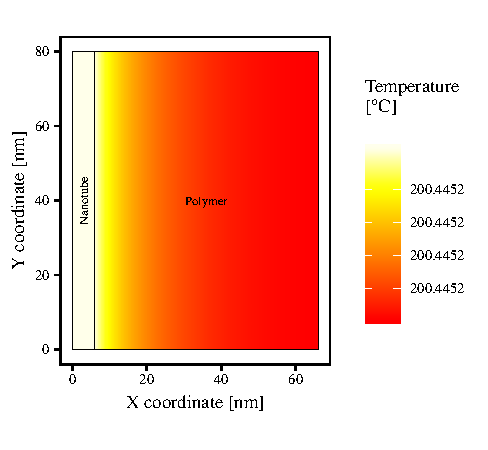
\includegraphics[width=0.45\textwidth]{resultats_comsol_axisymetrique_temp.pdf}
	} \qquad
	\subfigure[]
	{\label{fig:results_axysymmetric_b}
		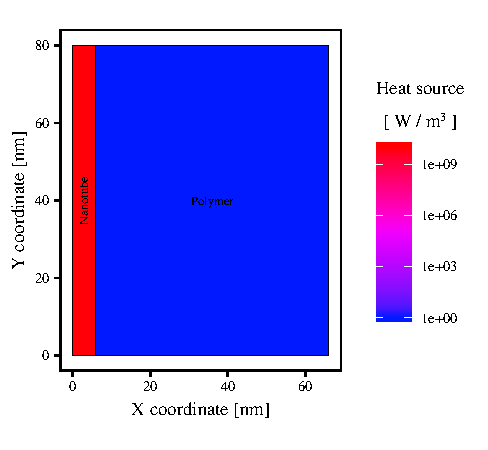
\includegraphics[width=0.45\textwidth]{resultats_comsol_axisymetrique_puissance.pdf}
	}
	\caption{Results of the FEM evaluating the heat generation within the MWCNT. The uniform temperature field is due to the short time constant for thermal diffusion in the model (see section \ref{sec:timeconstant}). a) uniform temperature field, b) heat generation field \cite{Brassard2018_figshare_article1}}
	\label{fig:results_axysymmetric}
\end{figure}

For the second FEM, the primary heat source was located at the contact point between the MWCNTs (Fig. \ref{fig:results_3D}b). 
Contribution from Joule heating within the MWCNTs was also present in the model with a power density 4 orders of magnitude lower. 
A uniform temperature profile is seen in MWCNTs, which is due to their high thermal conductivity. 
A uniform temperature of \SI{181}{\celsius} is obtained for this simulation after \SI{5}{\second} under an electric field of \SI{100}{\volt\per\metre}. 

\begin{figure}[h!]
	\centering
	\subfigure[]
	{\label{fig:results_3D_a} 								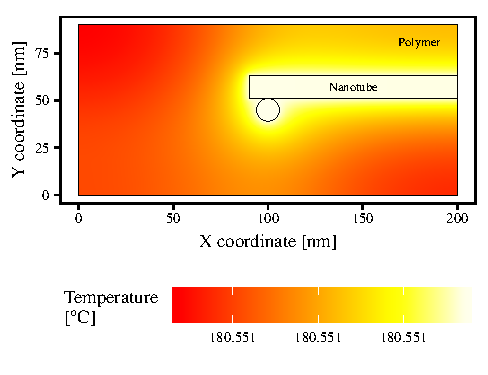
\includegraphics[width=0.45\textwidth]{resultats_comsol_3D_temp.pdf}
	} \qquad
	\subfigure[]
	{\label{fig:results_3D_b}
		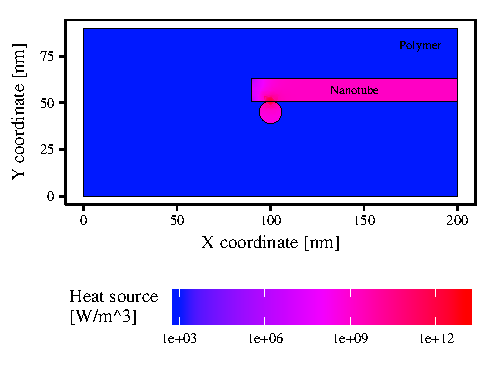
\includegraphics[width=0.45\textwidth]{resultats_comsol_3D_puissance_log.pdf}
	}
	\caption{Results of the FEM evaluating the effect of charge concentration and contact resistance. The uniform temperature field is due to the short time constant for thermal diffusion in the model (see section \ref{sec:timeconstant}) \cite{Brassard2018_figshare_article1}}
	\label{fig:results_3D}
\end{figure}
\FloatBarrier

In the third FEM, heat generation occurred almost exclusively in the polymer matrix (Fig. \ref{fig:result_gap}a and \ref{fig:result_gap}b). 
Heat is generated in the bulk of the polymer and a uniform temperature profile is obtained in the model (Fig. \ref{fig:result_gap}c and \ref{fig:result_gap}d). 

The third model demonstrates that the electric field required to reach a temperature similar to that of the first two models increases sharply when a small gap is introduced in the conductive network (Fig. \ref{fig:result_gap}). 
A gap of \SI{0.1}{\nano\metre}, between adjacent MWCNTs, required a field of \SI{9e9}{\volt\per\metre} to produce a temperature of \SI{185}{\celsius} (Fig. \ref{fig:result_gap}c). 
When the gap was increased to \SI{8}{\nano\metre} a field of \SI{5e10}{\volt\per\metre} was necessary to reach a similar temperature (Fig. \ref{fig:result_gap}d). 
These electrical field intensities are superior to the dielectric strength of PEI (\SI{3.3e7}{\volt\per\metre}) and the current went through the bulk of the polymer matrix. 
That seven order of magnitude increase in the electrical field, when a gap is introduced, confirms that the third heating mode is unlikely in practical applications. 
A connected network of MWCNTs provides pathways of lower resistance for the electrons to flow. 
A sharp increase in the resistance is indicative of a perturbation in the percolated network. 

\begin{figure}[h!]
	\centering
	\subfigure[]
	{\label{fig:result_gap_a} 								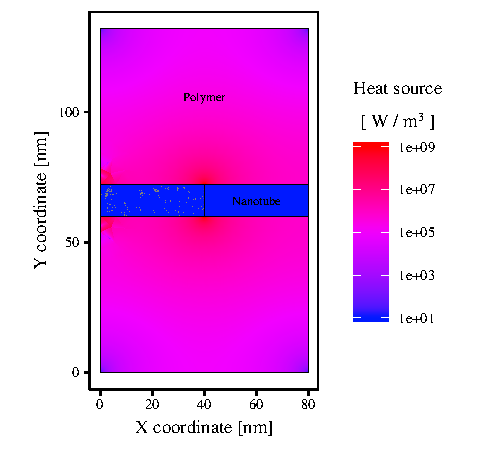
\includegraphics[width=0.46\textwidth]{resultats_0,1nm_comsol_2D_puissance.pdf}
	} 
	\subfigure[]
	{\label{fig:result_gap_b}
		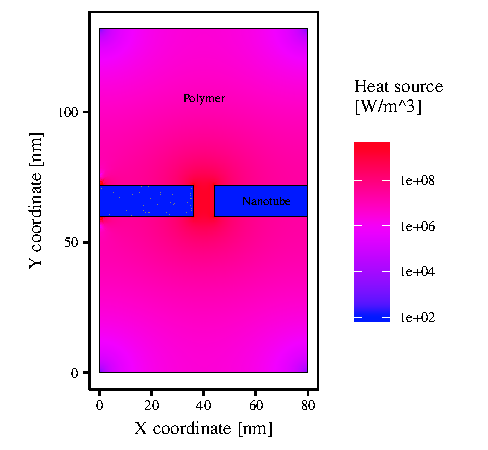
\includegraphics[width=0.46\textwidth]{resultats_8nm_comsol_2D_puissance.pdf}
	} \\
	\subfigure[]
	{\label{fig:result_gap_c} 								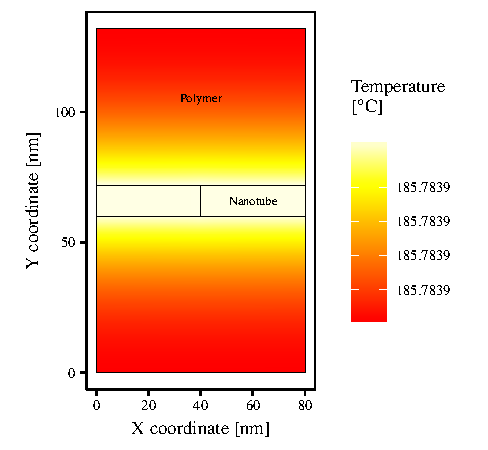
\includegraphics[width=0.46\textwidth]{resultats_0,1nm_comsol_2D_temp.pdf}
	} 
	\subfigure[]
	{\label{fig:result_gap_d}
		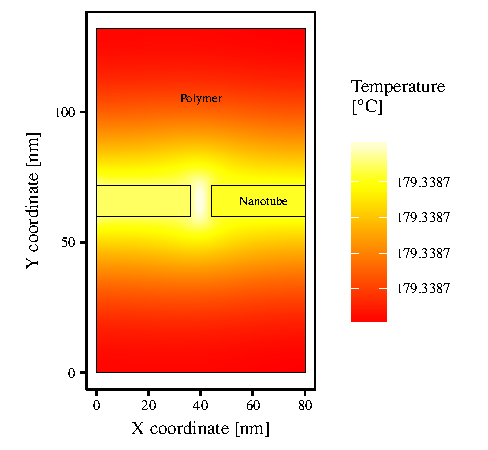
\includegraphics[width=0.46\textwidth]{resultats_8nm_comsol_2D_temp.pdf}
	}
	\caption{Effect of the gap length on the heat generation (a,b) and temperature fields (c,d) in the case of heat generation within the polymer. The uniform temperature fields are due to the short time constant for thermal diffusion in the model (see section \ref{sec:timeconstant}).  a) \SI{0.1}{\nano\metre} gap, \SI{9e9}{\volt\per\metre}, b) \SI{8}{\nano\metre} gap, \SI{5e10}{\volt\per\metre}, c) \SI{0.1}{\nano\metre} gap, \SI{9e9}{\volt\per\metre}, d) \SI{8}{\nano\metre} gap, \SI{5e10}{\volt\per\metre} \cite{Brassard2018_figshare_article1}}
	\label{fig:result_gap}
\end{figure}

From these results, we observe that conduction (and thus heat dissipation) within MWCNTs and through their contact points is the main driver for heat generation within a nanocomposite heating element. 
The uniform temperature fields observed at the constituent level lead to the conclusion that under normal operating conditions, local thermal degradation should not occur within the nanocomposite during the welding process. 

%%%%%%%%%%%%%%%%%%%%%%%%%%%%%%%%%%%%%%%%%%%%%%%%%%%%%%%%%%%%%%
\FloatBarrier
\subsection{Timescale analysis}
%%%%%%%%%%%%%%%%%%%%%%%%%%%%%%%%%%%%%%%%%%%%%%%%%%%%%%%%%%%%%%
\label{sec:timeconstant}

A comparative numerical analysis of the timescales for thermal diffusion, providing an explanation for the uniform temperature fields observed in the models, is presented in this section. 
Although PEI has poor thermal conductivity, uniform temperature fields with temperature variations not exceeding \SI{1e-5}{\celsius} are observed in the models. 
A comparative numerical analysis of the timescales for thermal diffusion, can explain this behaviour. 
This timescale is evaluated using the time constant for thermal diffusion ($t_D$) : 

\begin{equation}
t_D = \frac{L^2}{\alpha}
\label{equa:time_constant}
\end{equation}

\begin{figure}[htb]
	\center
	\captionsetup{width=35mm}
	%\resizebox{35mm}{!}{%\\
	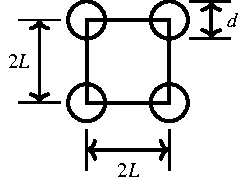
\includegraphics[scale=1]{arrangement_carre}
	%\tikzsetnextfilename{arrangement_carre}
	%\input{Tikz/arrangement_carre.tex}
	%}
	\caption{Square packing micromechanic model \cite{Brassard2018_figshare_article1}}
	\label{fig:square_packing}
\end{figure}

Assuming a uniform square packing of evenly distributed particles (Fig. \ref{fig:square_packing}) of known diameter ($d$) and variable volume fractions ($v_f$), it is possible to evaluate the average half distance ($L$) between particles :

\begin{equation}
L = \sqrt{\frac{\pi \ d^2}{16 \ v_f}}
\label{equa:L_average}
\end{equation}

The thermal diffusivity ($\alpha$) is defined as a function of thermal conductivity ($k$), density ($\rho$) and specific heat ($C_p$) : 

\begin{equation}
\alpha = \frac{k}{\rho \ C_p}
\label{equa:thermal_diffusivity}
\end{equation}

\begin{table}[htb]
	\centering
	\caption{Timescale for heat conduction}
	\begin{tabular}{@{}p{2.8cm}p{3.0cm}p{2.2cm}p{3.2cm}@{}}
		\toprule
		Weight fraction of MWCNTs & Volume fraction of MWCNTs & Average half distance & \textbf{Time constant}     \\
		$w_f$                     & $v_f$                     & L                     & $\mathbf{t_D}$             \\
		{[}\%{]}                  & {[}\%{]	}                 & {[}nm{]}              & \textbf{{[}s{]}}           \\ \midrule
		1                         & 0.65                      & 65.8                  & $\mathbf{3\times 10^{-8}}$ \\
		5                         & 3.31                      & 29.2                  & $\mathbf{6\times 10^{-9}}$ \\
		10                        & 6.74                      & 20.5                  & $\mathbf{3\times 10^{-9}}$ \\
		16                        & 11.02                     & 16.0                  & $\mathbf{2\times 10^{-9}}$ \\ \bottomrule
	\end{tabular}
	\label{tab:results_timescale}
\end{table}

Since the thermal conductivity of MWCNTs is very high compared to the polymer, only the properties of the matrix were considered in this timescale analysis. 
Table \ref{tab:results_timescale} presents the time constants calculated for thermal diffusion within the polymer matrix. 
The time constants varied from $3 \times 10^{-8}$ to \SI{2e-9}{\second} for $v_f$ varying from 1\% to 16\%. 
Considering that the simulations looked at Joule heating on a scale closer to the second, the short timescales for thermal diffusion explain the constant temperature fields. 

%%%%%%%%%%%%%%%%%%%%%%%%%%%%%%%%%%%%%%%%%%%%%%%%%%%%%%%%%%%%%%
\subsection{FTIR results}
%%%%%%%%%%%%%%%%%%%%%%%%%%%%%%%%%%%%%%%%%%%%%%%%%%%%%%%%%%%%%%

We collected FTIR spectra from a virgin PEI pellet, a nanocomposite PEI/MWCNT pellet, a nanocomposite film and two spectra from a fracture surface of a welded zone. 
The resulting absorbances spectra were calculated. 
The appearance of characteristic peaks, their position and width remained the same between the different spectra. 

\begin{figure}[h!]
	\center
	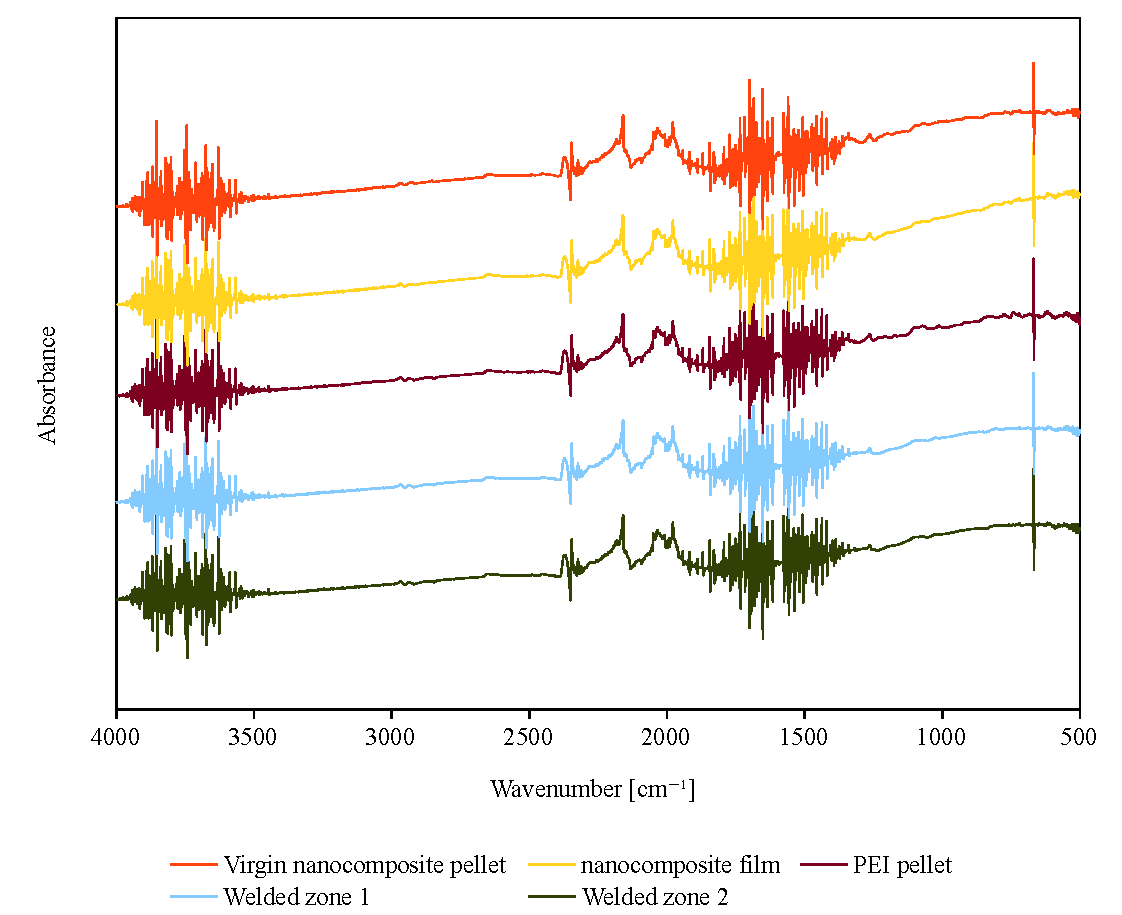
\includegraphics[width=0.8\textwidth]{FTIR_spectra.pdf}
	\caption{Raw FTIR spectra \cite{Brassard2018_figshare_article1}}
	\label{fig:FTIR_spectra}
\end{figure}

%%%%%%%%%%%%%%%%%%%%%%%%%%%%%%%%%%%%%%%%%%%%%%%%%%%%%%%%%%%%%%%%%%
\Annexe{Informations complémentaires au chapitre 5}
%%%%%%%%%%%%%%%%%%%%%%%%%%%%%%%%%%%%%%%%%%%%%%%%%%%%%%%%%%%%%%%%%%

Cette annexe a été soumise en accompagnement du second article. 

%%%%%%%%%%%%%%%%%%%%%%%%%%%%%%%%%%%%%%%%%%%%%%%%%%%%%%%%%%%%%%%%%
\section{Supplementary Information}
%%%%%%%%%%%%%%%%%%%%%%%%%%%%%%%%%%%%%%%%%%%%%%%%%%%%%%%%%%%%%%%%%

This section presents a summary of all the materials properties used in the model. 

The relative permittivity for the PEI/MWCNT nanocomposite was calculated with the law of mixture from the reported value of 3.15 for SABIC’s PEI grade ULTEM 1010 and a relative permittivity of 15 for MWCNTs \cite{Katsounaros2011}. 

% Please add the following required packages to your document preamble:
% \usepackage{booktabs}
\begin{table}[ht]
	\centering
	\caption{List of all specific heat used in the model}
	\resizebox{\textwidth}{!}{
		\begin{tabular}{@{}cccccc@{}}
			\toprule
			Temperature & CF/PEEK    & PEI/MWCNT  & Alumina Silicate & Copper     & GPO3       \\
			{[}$^{\circ}$C{]} & {[}J\,kg$^{-1}$\,K$^{-1}${]} & {[}J\,kg$^{-1}$\,K$^{-1}${]} & {[}J\,kg$^{-1}$\,K$^{-1}${]}  & {[}J\,kg$^{-1}$\,K$^{-1}${]} & {[}J\,kg$^{-1}$\,K$^{-1}${]} \\ \midrule
			
			Constant    &            &            &                  & 385        & 1260       \\
			40          & 926        & 1059       &                  &            &            \\
			97          &            &            & 975              &            &            \\
			139         & 1265       &            &                  &            &            \\
			159         & 1359       &            &                  &            &            \\
			207         &            & 1561       &                  &            &            \\
			227         &            & 1765       &                  &            &            \\
			310         & 1809       &            &                  &            &            \\
			343         & 2400       &            &                  &            &            \\
			360         & 1792       &            &                  &            &            \\
			399         & 1790       & 1955       &                  &            &            \\ \midrule
			Source      & Measured   & Measured   & Measured         & COMSOL     & Suppliers  \\ \bottomrule
	\end{tabular} }
	\label{tab:SI2_table1}
\end{table}

\begin{table}[ht]
	\centering
	\caption{List of all thermal conductivity used in the model}
	\resizebox{\textwidth}{!}{%
		\begin{tabular}{@{}ccccccc@{}}
			\toprule
			Temperature & CF/PEEK   & CF/PEEK       & PEI/MWCNT & Alumina   & Copper    & GPO3      \\
			& Parallel  & Perpendicular &           & Silicate  &           &           \\
			{[}$^{\circ}$C{]} & {[}W\,m$^{-1}$\,K$^{-1}${]} & {[}W\,m$^{-1}$\,K$^{-1}${]} & {[}W\,m$^{-1}$\,K$^{-1}${]} & {[}W\,m$^{-1}$\,K$^{-1}${]} & {[}W\,m$^{-1}$\,K$^{-1}${]} & {[}W\,m$^{-1}$\,K$^{-1}${]} \\ \midrule
			Constant    &           &               &           & 5.7       & 400       & 0.27      \\
			20          & 2.25      & 0.55          & 0.41      &           &           &           \\
			40          &           &               & 0.30      &           &           &           \\
			60          &           &               & 0.43      &           &           &           \\
			110         &           &               & 0.46      &           &           &           \\
			150         &           &               & 0.48      &           &           &           \\
			200         & 3.02      & 0.73          &           &           &           &           \\ \midrule
			Source      & Measured  & Measured      & Measured  & Measured  & COMSOL    & Suppliers \\ \bottomrule
		\end{tabular}%
	}
	\label{tab:SI2_table2}
\end{table}

% Please add the following required packages to your document preamble:
% \usepackage{booktabs}
% \usepackage{graphicx}
\begin{table}[ht]
	\centering
	\caption{List of all densities used in the model}
	\resizebox{\textwidth}{!}{%
		\begin{tabular}{@{}llllll@{}}
			\toprule
			Temperature       & CF/PEEK            & PEI/MWCNT          & Alumina Silicate   & Copper             & GPO3               \\
			{[}$^{\circ}$C{]} & {[}kg\,m$^{-3}${]} & {[}kg\,m$^{-3}${]} & {[}kg\,m$^{-3}${]} & {[}kg\,m$^{-3}${]} & {[}kg\,m$^{-3}${]} \\ \midrule
			Constant          &                    & 1320               & 2500               & 8700               & 1800               \\
			0                 & 1601               &                    &                    &                    &                    \\
			50                & 1598               &                    &                    &                    &                    \\
			100               & 1593               &                    &                    &                    &                    \\
			150               & 1586               &                    &                    &                    &                    \\
			200               & 1575               &                    &                    &                    &                    \\
			250               & 1563               &                    &                    &                    &                    \\
			300               & 1551               &                    &                    &                    &                    \\
			350               & 1537               &                    &                    &                    &                    \\
			400               & 1524               &                    &                    &                    &                    \\ \midrule
			Source            & \cite{Talbot2013}  & Measured           & Measured           & COMSOL             & Suppliers          \\ \bottomrule
		\end{tabular}%
	}
	\label{tab:SI2_table3}
\end{table}

\begin{table}[ht]
	\centering
	\caption{List of electrical properties for the model}
	\begin{tabular}{@{}lccccc@{}}
		\toprule
		&                   & \multicolumn{2}{c}{PEI/MWCNT} & \multicolumn{2}{c}{Copper}  \\ \midrule
		Electrical conductivity & {[}S\,m$^{-1}${]} & 80         & Measured         & $5.998 \times 10^7$ & COMSOL \\
		Relative permittivity   & {[} \ {]}         & 4.3        & Calculated       & 1                  & COMSOL \\ \bottomrule
	\end{tabular}%
	\label{tab:SI2_table4}
\end{table}

\FloatBarrier